\documentclass{ximera}

\makeatletter

\RequirePackage{sagetex}


\graphicspath{
  {./}
  {./explorePolynomials/}
  {./exploreRadicals/}
  {./graphing/}
  {./examReview}
}


%% Because log being natural log is too hard for people.
\let\logOld\log% Keep the old \log definition, just in case we need it.
\renewcommand{\log}{\ln}


\providecommand\tabitem{\makebox[1em][r]{\textbullet~}}
\providecommand{\letterPlus}{\makebox[0pt][l]{$+$}}
\providecommand{\letterMinus}{\makebox[0pt][l]{$-$}}

\renewcommand{\texttt}[1]{#1}% Renew the command to prevent it from showing up in the sage strings for some weird reason.


%%%%%%%%%%%%%%%%%%%%%%%%%%%%%%%%
%%% Randomize Locations Code %%%
%%%%%%%%%%%%%%%%%%%%%%%%%%%%%%%%

%% Required Packages
%\RequirePackage[margin=2.5cm]{geometry}% Set generic Margins to 1.5cm
\RequirePackage{fancyhdr}% Used to make header/footers
%\RequirePackage[hidelinks]{hyperref}%
%\RequirePackage{tikz, pgfplots}
\RequirePackage{forloop}
\RequirePackage{changepage}
\RequirePackage{morewrites}
\RequirePackage{calc}


%%%%%%%%%%%%%%%%%%%%%%%% End of Required Packages



%% Necessary Counters

\newcounter{choiceNum}% This will track the choice number in a given MCChoice environment.
\newcounter{choiceEnvNum}% This lets the \choice generated commands be uniquely identified to the correct MCChoice environment.
    \setcounter{choiceEnvNum}{0}% Start at 0 as we step the counter before assigning things.
\newcounter{questionNum}% Tracks what number a question is within a given MCQ environment.



% Iteration counters
\newcounter{Iteration@printChoices}
\newcounter{Iteration@questionsInBlock}
\newcounter{Iteration@printQuestions}

%% End Counters

%% New "if" commands
\newif\ifVerbose% For error Checking
\Verbosefalse

\newif\ifInner@Shuffle% If we want our vector to be shuffled
\Inner@Shufflefalse

\newif\ifInner@OrderForward% If we want non-shuffled and original order (smallest value to biggest value).
\Inner@OrderForwardfalse

\newif\ifInner@OrderReverse% If we want non-shuffled but reverse order (biggest value to smallest value).
\Inner@OrderReversefalse

\newif\ifshuffleChoices%    Toggle to shuffle choice locations.
\shuffleChoicesfalse

\newif\ifshuffleQuestions%  Toggle to shuffle Question locations.
\shuffleQuestionsfalse

\newif\ifgenAnsKey% Tracks if we want 
\genAnsKeyfalse

\newif\ifcorrectAns% This will track if a choice is correct.
\correctAnsfalse

%% End "if" commands


%%%%%%%%%%%%%%%%%%%%%%%% End of Package Options


%%% Support commands %%%
\providecommand\compareStrings[2]{% Used to compare two strings to see if they are the same - up to case sensitivity.
    \edef\tempA{\lowercase{\noexpand\ifnum0=\noexpand\pdfstrcmp
        {\noexpand\zap@space#1 \noexpand\@empty}%
        {\noexpand\zap@space#2 \noexpand\@empty}%
    }\relax}%
    \tempA
        \expandafter\@firstoftwo
    \else
        \expandafter\@secondoftwo
    \fi
}

\providecommand{\MakeCounter}[1]{%% Code located in "Utilitymacros.dtx"
  \@ifundefined{c@#1}% Check to see if counter exists
        {     % If not, create it and set it to 0.
            \newcounter{#1}
            \setcounter{#1}{0}
        }
        {%If so, reset to 0.
            \setcounter{#1}{0}
        }
    }








%%%%%%%%%%%%%%%%%%%%%%%%%%%%%%%%%%%%%%%%%%%%%%%%%%%%%%%%%%%%%%%%%%%%%
%%%%%%%%%%%%%%%%%%%		  Randomize Commands		%%%%%%%%%%%%%%%%%
%%%%%%%%%%%%%%%%%%%%%%%%%%%%%%%%%%%%%%%%%%%%%%%%%%%%%%%%%%%%%%%%%%%%%


%%%%%%%%%%%%%%%%%%%%%%%%%%%%%%%%%%%%%%%%%%%%%%%%%%%%%%%%%%%%%
%%%%%%%%%%%%  Random Permutation Command  %%%%%%%%%%%%%%%%%%%
%%%%%%%%%%%%%%%%%%%%%%%%%%%%%%%%%%%%%%%%%%%%%%%%%%%%%%%%%%%%%

\MakeCounter{RndQuant}%		        Tracks the number of desired counters
\MakeCounter{Temp@Hold}%		    Temp counter to hold the command value because tex is weird.
\MakeCounter{Temp@RandMe}%	        Temp counter like previous.

\providecommand*\ifcounter[2]{%         Function checks if a counter named #1 exists. If not it creates it. After existance is confirmed (or implemented), set the counter to #2.
  \ifcsname c@#1\endcsname
  \else
    \MakeCounter{#1}
  \fi
\setcounter{#1}{#2}
}

\providecommand{\RandMe}[3]{% #1 is the max number for range, #2 is the name of the counter to hold the list, and #3 is how many from that list to generate. Thus \RandMe{100}{TEMP}{5} will generate 5 counters, named \TEMPI, \TEMPII, \TEMPIII, \TEMPIV, \TEMPV. Each of which will have a (unique) number between 1 and 100.

    %Assign a maximum on how many numbers to pick. Set default to the max list size, and save in counter "RndQuant"
    \ifthenelse{\isempty{#3}}
        {
        \setcounter{RndQuant}{#1+1}
        }
        {
        \setcounter{RndQuant}{#3+1}
        }

    %Generate a starting list of numbers 1 to maximum number given
    \forloop{Iteration1}{1}{\arabic{Iteration1} < \arabic{RndQuant}}{
        \ifcounter{#2\Roman{Iteration1}}{\arabic{Iteration1}}
        }% End Forloop
    
    
    %Permute using Knuth method
    \forloop{Iteration1}{1}{\arabic{Iteration1} < \arabic{RndQuant}}{
        \@genrand{TempRandMe}{\arabic{Iteration1}}{#1}
    
        \ifcounter{Temp@RandMe}{\TempRandMe}
        \ifcounter{Temp@Hold}{\arabic{#2\Roman{Temp@RandMe}}}
        
        \ifcounter{#2\Roman{Temp@RandMe}}{\arabic{#2\Roman{Iteration1}}}
        \ifcounter{#2\Roman{Iteration1}}{\arabic{Temp@Hold}}
    }
}




%%%%%%%%%%%%%%%%%%%%%%%%%%%%%%%%%%%%%%%%%%%%%%%%%%%%%%%%%%%%%
%%%%%%%%%%%%  Random Permutation Command  %%%%%%%%%%%%%%%%%%%
%%%%%%%%%%%%%%%%%%%%%%%%%%%%%%%%%%%%%%%%%%%%%%%%%%%%%%%%%%%%%


\providecommand{\@genrand}[3]{%\@genrand{NAME}{MIN}{MAX} generates a random number before MIN and MAX and stores it in the command \NAME. 
    \expandafter\pgfmathrandominteger\csname #1\endcsname{#2}{#3}
    \setcounter{#1}{\csname #1\endcsname}
}




%%%%%%%%%%%%%%%%%%%%%%%%%%%%%%%%%%%%%%%%%%%%%%%%%%%%%%%%%%%%%%%%%%%%%%%%%%%%%%%
%%%%%%%%%  		Make Vector is used to generate most random lists		%%%%%%%%%
%%%%%%%%%%%%%%%%%%%%%%%%%%%%%%%%%%%%%%%%%%%%%%%%%%%%%%%%%%%%%%%%%%%%%%%%%%%%%%%

\MakeCounter{Temp@1}
\MakeCounter{Temp@2}
\MakeCounter{Temp@3}
\MakeCounter{Iteration@1}
\MakeCounter{Iteration@2}
\MakeCounter{Iteration@3}
\MakeCounter{Iteration@4}
\MakeCounter{Placement@1}
\setcounter{Placement@1}{1}



%%%%%%%% Internal Keys
%% These are to use for internal flags only.
\providecommand{\inner@SetKeys}[1]{
\setkeys{key@Inner}{InnerShuffle={}, Order@Direction={},#1}
}


\define@key{key@Inner}{InnerShuffle}{% This flag is for shuffling questions.
\ifthenelse{\equal{#1}{true}}
	{
	\Inner@Shuffletrue
	}
	{
	\Inner@Shufflefalse
	}
}

\define@key{key@Inner}{Order@Direction}{% This flag gives the order in which vectors are saved.
\ifthenelse{\equal{#1}{forward}}
	{
	\Inner@OrderForwardtrue
	}
	{
	\Inner@OrderForwardfalse
	}
\ifthenelse{\equal{#1}{reverse}}
	{
	\Inner@OrderReversetrue
	}
	{
	\Inner@OrderReversefalse
	}
}



\providecommand{\make@Vector}[5][InnerShuffle=false, Order@Direction=forward]{% This is to make either an ordered or a shuffled list of values
	% #1 is optional and is for internal flags. 
	% #2 is the name of the output counters
	% #3 is the minimum counter value
	% #4 is the maximum counter value
	% #5 is the number of desired counters.
	% Counters will be saved as #2\Roman{#}
	
	\inner@SetKeys{#1}% Set any given keys
	% Possible flags:
		% InnerShuffle flag "true" will shuffle, "false" won't
		% Order@Direction; "forward" will list questions in increasing order. "reverse" will list the questions in 					decreasing order
		% 
	
%%%%%%%%%%%%%%%%%%%%%%%%%%%%%%%%%%%%%%%%%%%%%%%%%%%%%%%%%%%%%%%%%%%%%%%%%%%%%%%
%%%%%%%%%  		First we will choose and order the initial values		%%%%%%%%%
%%%%%%%%%%%%%%%%%%%%%%%%%%%%%%%%%%%%%%%%%%%%%%%%%%%%%%%%%%%%%%%%%%%%%%%%%%%%%%%
	\setcounter{Temp@1}{#4}
	\addtocounter{Temp@1}{-#3}
	\ifnum #5 = \value{Temp@1}% The special case where we want all the values. Randomizing into a full list just to order it is silly so we deal with this case separately.
		\forloop{Iteration@1}{1}{\arabic{Iteration@1} < \arabic{Temp@1}}
			{% Start of forloop
			\MakeCounter{Ordered@\Roman{Iteration@1}}	% Check to see if counter exists
			\MakeCounter{C@Shuffle\Roman{Iteration@1}}
			\setcounter{Ordered@\Roman{Iteration@1}}{\arabic{Iteration@1}}
			\setcounter{C@Shuffle\Roman{Iteration@1}}{\arabic{Iteration@1}}
			}
	\else% If we don't want a full list, then we need to choose some.
		\setcounter{Temp@1}{#5}% Track how many numbers we want.
		\stepcounter{Temp@1}% Step for the < sign
		\forloop{Iteration@1}{1}{\arabic{Iteration@1} < \arabic{Temp@1}}
			{% Start of forloop
	
			\MakeCounter{Ordered@\Roman{Iteration@1}}	% Check to see if counter exists
			\MakeCounter{CTemp\Roman{Iteration@1}}	% Check to see if counter exists
			\MakeCounter{C@Shuffle\Roman{Iteration@1}}
		
			\@genrand{Temp@2}{#3}{#4}
			\ifVerbose{Your first choice for the question number is \arabic{Temp@2}}\\ \fi
			\forloop{Iteration@2}{1}{\arabic{Iteration@2} < \arabic{Iteration@1}}
				{% Start of inner forloop. This loop checks for uniqueness of counter value.
				\ifnum\value{Temp@2}=\value{CTemp\Roman{Iteration@2}}% Check to see if the counter matches any previous counter
				\@genrand{Temp@2}{#3}{#4}% If so, fix it.
				\setcounter{Iteration@2}{0}% Reset the check counter so we can check if the new number is used.
				\ifVerbose Your revised choice for the number is \arabic{Temp@2} \\ \fi
				\fi
	%			\arabic{Iteration@2}, \arabic{CTemp\Roman{Iteration@2}}\\
				}% 
			
			\setcounter{CTemp\Roman{Iteration@1}}{\arabic{Temp@2}}% Save (unsorted) unique value in a temp list of variables.
			\setcounter{C@Shuffle\Roman{Iteration@1}}{\arabic{Temp@2}}% Save (unsorted) unique value in a temp list of variables. This one is to be used in the case we want shuffled values at the end.
		
			\ifVerbose (Unordered) We want questions number \arabic{Temp@2} \fi
		
			}
		% Now we want to sort the list	
	
		\forloop{Iteration@3}{1}{\arabic{Iteration@3}<\arabic{Temp@1}}
			{% For each variable
				\setcounter{Placement@1}{1}% Default the placeholder counter to some gigantic number so I can proceed to find the smallest possible number.
			
				\forloop{Iteration@4}{1}{\arabic{Iteration@4}<\arabic{Temp@1}}
					{
					\ifnum\value{CTemp\Roman{Iteration@4}}<\value{CTemp\Roman{Placement@1}}
						\setcounter{Placement@1}{\arabic{Iteration@4}}% Keep track of which counter was the largest so far
					\fi
					}
	
				\setcounter{Ordered@\Roman{Iteration@3}}{\arabic{CTemp\Roman{Placement@1}}}% Set the final counter.
				\setcounter{CTemp\Roman{Placement@1}}{999999}% Now remove that place as a viable option for next run.
				\ifVerbose (Ordered) We want question number \arabic{Ordered@\Roman{Iteration@3}} \fi
			}
	\fi	
%%%%%%%%%%%%%%%%%%%%%%%%%%%%%%%%%%%%%%%%%%%%%%%%%%%%%%%%%%%%%%%%%%%%%%%%%%%%%%%	
%%%%%%%%%%%		Finished Choosing and ordering initial values		%%%%%%%%%%%
%%%%%%%%%%%%%%%%%%%%%%%%%%%%%%%%%%%%%%%%%%%%%%%%%%%%%%%%%%%%%%%%%%%%%%%%%%%%%%%
%%%%%%%%%%%   		Now reorder and assign final names				%%%%%%%%%%%
%%%%%%%%%%%%%%%%%%%%%%%%%%%%%%%%%%%%%%%%%%%%%%%%%%%%%%%%%%%%%%%%%%%%%%%%%%%%%%%
	
	
	\ifInner@OrderReverse
		\setcounter{Temp@3}{#5}
		\forloop{Iteration@1}{1}{\arabic{Iteration@1} < \arabic{Temp@1}}
			{
			\MakeCounter{#2\Roman{Iteration@1}}% Make the counter if it doesn't exist.
			\setcounter{#2\Roman{Iteration@1}}{\arabic{Ordered@\Roman{Temp@3}}}% Set the final counter version to the current "last" unused value.
			\addtocounter{Temp@3}{-1}% Decrement the counter for next assignment
			}
	\else% If we aren't doing it in reverse, assume we want forward order. This is default.
		\forloop{Iteration@1}{1}{\arabic{Iteration@1} < \arabic{Temp@1}}
			{
			\MakeCounter{#2\Roman{Iteration@1}}% Make the counter if it doesn't exist.
			\setcounter{#2\Roman{Iteration@1}}{\arabic{Ordered@\Roman{Iteration@1}}}% Set the final counter version to the next value.
			}
	
	\fi% End of forward/reverse order version

	\ifInner@Shuffle
		\forloop{Iteration@1}{1}{\arabic{Iteration@1} < \arabic{Temp@1}}
			{
			\MakeCounter{#2\Roman{Iteration@1}}% Make the counter if it doesn't exist.
			\setcounter{#2\Roman{Iteration@1}}{\arabic{C@Shuffle\Roman{Iteration@1}}}% Set the counter to the next value.
			}

	\fi% End of Shuffle order version
	
}


%%%%%%%%%%%%%%%%%%%%%%%%%%%%%%%%%%%%%%%%%%%%%%%%%%%%%%%%%%%%%%%%%%%%%%%%%%%%%%%%%%%%%%%%%%%%%%%%%%%%
%%%%%%%%%%%%%%%%%%%%%%%%%               Shuffle Structure               %%%%%%%%%%%%%%%%%%%%%%%%%%%%
%%%%%%%%%%%%%%%%%%%%%%%%%%%%%%%%%%%%%%%%%%%%%%%%%%%%%%%%%%%%%%%%%%%%%%%%%%%%%%%%%%%%%%%%%%%%%%%%%%%%
%%%%% Structure of randomizing/printing problems and choices:
%    All the MC questions are wrapped in an environment, eg MCQuestions. 
%        At the termination of the block, the questions are printed. This will determine shuffling.
%    We use a \questionblock type command to save questions together that need to be put together. 
%        eg questions that have a ``use the following information for the next 3 problems.''
%        \shuffleblock takes an argument that denotes how many sub-questions are contained in a block.
%    We use a \question command to save the content of a question into a macro.
%    Each individual MC question uses a choices environment and choices command as the \item equivalent.
%        The termination of the choices environment will shuffle (or not) the choices.
%
%    When we print the problems, we will iterate through the question content and/or the shuffleblocks
%        If a shuffle block has too many questions in it for how many ``more'' questions we want, we skip it.
%        Print things in order (or random order) until we have however many questions we want.
%            BADBAD:: If you randomize the questions just right with larger shuffle blocks at the end;
%                it's possible that the number of problems printed won't be the desired amount, even if there
%                are enough problems in the bank. We can get around this by changing the seed in the short term.
    


%%%%%%%%%%%%%%%%%%%%%%%%%%%%%%%%%%%%%%%%%%%%%%%%%%%%%%%%%%%%%%%%%%%%%%%%%%%%%%%%%%%%%%%%%%%%%%%%%%%%
%%%%%%%%%%%%%%%%%%%%%%%%%       Question Environments and Commands      %%%%%%%%%%%%%%%%%%%%%%%%%%%%
%%%%%%%%%%%%%%%%%%%%%%%%%%%%%%%%%%%%%%%%%%%%%%%%%%%%%%%%%%%%%%%%%%%%%%%%%%%%%%%%%%%%%%%%%%%%%%%%%%%%

%% MCQuestions Environment
\newcounter{MCquestionPrint}% Counter to save how many questions we want to print from the MCQ environment.

\newenvironment{MCQuestions}[1][1000]% Use massive default number to print all problems if none is given.
    {% Start environment code
        \setcounter{MCquestionPrint}{#1}%   Save how many questions we want from this environment to a counter.
    }% End start environment code
    {% End environment code
        {\expandafter\printQuestions{\arabic{MCquestionPrint}}}%
    }% End of end environment code.





%%% Defining the questionblock command.
\newif\ifquestionBlock%     We define a flag so we know if we are in a question block.
\questionBlockfalse%        We will assume that, by default, we are not in a question block.
\newcounter{shuffleNum}%    This will track how many blocks are present to shuffle.
\setcounter{shuffleNum}{0}%    Start at zero.
%\newcounter{blockNum}%      A counter to track which block number we are on.
%\setcounter{blockNum}{0}%   By default we haven't iterated a block yet.

\providecommand{\questionBlock}[2]{%    This is a command that should allow one to group together a block of questions, 
%                                            in order, to be considered one ``big question'' for the purposes of shuffle.
%                                        Syntax: #1 is the number of questions in the block
%                                                #2 is the actual content of the block, eg the questions.
    \stepcounter{shuffleNum}%                                   We have started a question block, so we iterate the shuffleNum to know we aim to shuffle this as one block. 
    \expandafter\MakeCounter{Block\roman{shuffleNum}Size}%      Create a counter to hold how many questions are in this block.
    \expandafter\setcounter{Block\roman{shuffleNum}Size}{#1}%   And record how many questions are in this block.
    \ifpoolProblem
        \stepcounter{poolPlacement}% Step this counter once to say we're adding one placement into the pool.
    \fi
    
    \expandafter\gdef\csname blockPosition\roman{shuffleNum}\endcsname{
        \questionBlocktrue% We are now in a question block, so we set the flag to true. 
    %                           This should change the ``\question" behavior to just display the questions.
        #2
        \questionBlockfalse% Toggle off the shuffle block once we have spit out the problems.
        }

}% End questionBlock definition

\DeclareRobustCommand{\question}[1]{ \begin{problem} #1 \end{problem}}


%% Defining the \question command.
\DeclareRobustCommand{\question}[1]{% Question command should contain a question to be formatted.
        \ifquestionBlock
        % If it's just a block on its own, then we just group them together as one large question and call it a day.
            \begin{problem} #1\end{problem}
        \else
            \stepcounter{shuffleNum}% A new question means we need to step current shuffle number count (before definition since counter starts at 0)
            \expandafter\gdef\csname blockPosition\roman{shuffleNum}\endcsname{\begin{problem} #1 \end{problem}}
        \fi
    
    }% End \question code


%% Define the print questions command.
\newcounter{questionsPrintNum}
\setcounter{questionsPrintNum}{0}
\providecommand{\printQuestions}[1]{% This is a command that will print questions that were defined in the current question environment.
    %First, we make the call the shuffle vector based on if we are shuffling these or not.
        \ifshuffleQuestions%                    If we are shuffling, then shuffle up the call
            \make@Vector[InnerShuffle=true]{questionLoc}{1}{\arabic{shuffleNum}}{\arabic{shuffleNum}}
        \else%                                  Otherwise, display them in original first to last order.
            \make@Vector[InnerShuffle=false,Order@Direction=forward]{questionLoc}{1}{\arabic{shuffleNum}}{\arabic{shuffleNum}}
        \fi	


    	\setcounter{questionsPrintNum}{#1}%     Record how many problems we need to print.
        \stepcounter{questionsPrintNum}%        The ifthenelse doesn't like <=, so we step the counter to avoid this problem.
        \stepcounter{shuffleNum}%               The forloop doesn't like <=, so we step the counter to avoid this problem.
    	% Now print the results:
        
        \forloop{Iteration@printQuestions}{1}{\arabic{Iteration@printQuestions}<\arabic{shuffleNum}}{% Begin forloop
            % Now we need to see if we need to print the next shuffle problem.
            %% First check to see if the next shuffle item is a question block by seeing if the block num counter is defined.
            \ifcsname c@Block\roman{questionLoc\Roman{Iteration@printQuestions}}Size\endcsname
                % If the counter is defined, then the next item is a question block and the counter is the number of questions.
                \ifthenelse{ \arabic{Block\roman{questionLoc\Roman{Iteration@printQuestions}}Size} < \arabic{questionsPrintNum}}
                    {% If the block is small enough, then go ahead and print them.
                        \ifVerbose Printing question block labeled: blockPosition\roman{questionLoc\Roman{Iteration@printQuestions}}...\fi
                        
                        \csname blockPosition\roman{questionLoc\Roman{Iteration@printQuestions}}\endcsname%
                        %   And, since we printed them, we need fewer problems to print!
                        \addtocounter{questionsPrintNum}{-\arabic{Block\roman{questionLoc\Roman{Iteration@printQuestions}}Size}}
                        
                        \ifVerbose Now we have \thequestionsPrintNum more questions to go...\fi
                    }
                    {% Otherwise, do nothing.
                        Tried to print a question block but it didn't fit...
                    }
            \else% Otherwise the next item is just a singleton question.
                %Printing question labeled: blockPosition\roman{questionLoc\Roman{Iteration@printQuestions}}
                
                \csname blockPosition\roman{questionLoc\Roman{Iteration@printQuestions}}\endcsname%
                \addtocounter{questionsPrintNum}{-1}% We printed a question, so there's one fewer needed to print.
                
                %Now we have \thequestionsPrintNum more questions to go...
            \fi
            %% Finally, we will check if we still need to use this for loop.
            \ifthenelse{\arabic{questionsPrintNum} < 2}{% If the questionsPrint is less than 2 (since we stepped the counter), then we are done.
            \setcounter{Iteration@printQuestions}{\arabic{shuffleNum}}% Breakout of the forloop.
            \ifVerbose And we're done.\fi
            }
            {% If we aren't done, then do nothing with this check.
            \ifVerbose Keep going, we haven't stopped yet...\fi
            }
        }% End forloop
        %\addtocounter{shuffleNum}{-1}% Undo the stepcounter to be safe.
    }% End \printQuestions code.


%%%%%%% Choices Code

%\let\choiceOnline\choice% Define the old online choice command as the generic ``choice'' command; we'll see what happens.
\providecommand{\choiceShuffle}[2][]{% Choice command holds a multiple choice option by generating a new command with unique name that will be used to write the outputs at the end of the MCChoices environment.
            \refstepcounter{choiceNum}% A new choice means we need to step current choice (before definition since counters starts at 0)
            \expandafter\gdef\csname \Roman{choiceEnvNum}choice\roman{choiceNum}\endcsname{\choice[#1]{#2}}
        }% End of \choice code.
        
%%% Choice environment just collects and prints choices for each one locally.
\newenvironment{choices}{% Start environment code for multiple choice Choices environment
        \setcounter{choiceNum}{0}% New MCChoices environment means a new set of choices, so reset current choice to 0.
        \refstepcounter{choiceEnvNum}
    }% End of end-environment code.
    {
    \printChoices
    }



\renewcommand{\thechoiceEnvNum}{\Roman{choiceEnvNum}}
\renewcommand{\thechoiceNum}{\Alph{choiceNum}}
\renewcommand{\theIteration@printChoices}{\Alph{Iteration@printChoices}}

\providecommand{\printChoices}{% \printChoices is an internal macro to print the choices at the end of a MCChoice environment, depending on if we want them shuffled or not.

    %First, we make the call vector based on if we are shuffling these or not.
    \ifshuffleChoices% If we are shuffling, then shuffle up the call
        \make@Vector[InnerShuffle=true]{choiceLoc}{1}{\arabic{choiceNum}}{\arabic{choiceNum}}
    \else% Otherwise, display them in original first to last order.
        \make@Vector[InnerShuffle=false, Order@Direction=forward]{choiceLoc}{1}{\arabic{choiceNum}}{\arabic{choiceNum}}
    \fi	
    
	% Now print the results:
	
    \stepcounter{choiceNum}% Step counter for the < symbol in foreloop.
    
    \ifVerbose I think my choice number is \thechoiceNum{} and my choice env is \thechoiceEnvNum{}\fi
    \begin{multipleChoice}
        \forloop{Iteration@printChoices}{1}{\arabic{Iteration@printChoices}<\arabic{choiceNum}}{% Begin forloop
                \csname \thechoiceEnvNum choice\expandafter\roman{choiceLoc\Roman{Iteration@printChoices}}\endcsname
            }% End For Loop
    \end{multipleChoice}
    }% End of \printChoices code.











\title{Exam Two Review}


\begin{document}
\begin{abstract}
This is a (lengthy) practice exam for Exam 2 on Polynomials.
\end{abstract}
\maketitle


\shuffleChoicestrue
\shuffleQuestionstrue
\pgfmathsetseed{223}

\textbf{NOTE:} There may be random lines that look like \verb|\texttt{(SOME TEXT)}| and maybe even some \verb|{ }| within that text. You can ignore everything that isn't the text itself; ie the texttt bit and the braces, they are an artifact of how some randomization is being done that I haven't had time to fix yet. If you literally delete the \verb|\texttt| and the braces from what you see, and just keep the text itself, it will read exactly as intended. So just ignore all those texttt and braces whenever you see them.

Also note: Some of the below has randomized elements, some do not. Currently Xronos does not support randomized graphing (although we're working on it!) so a lot of the graphing problems won't randomize, but a surprising amount of the other problems will change values or text if you hit the green ``another'' button in the top right corner to get another version of this practice exam. This also means it may take some time for the entire test to render because we have to rely on public servers to do the randomization for us currently, so please be patient. If it takes more than 3-5 minutes to fill out the random values (meaning: if there are still spinning wheels of death going after 3-5 minutes) there is a problem. Try hitting the ``another'' button to see if it resolves itself. If it keeps doing this, please contact your instructor and let him know!



%%% This is a bulk problem list for input into exams.
%%  Specifically this is on extrema of polynomials.
%       Includes things like identifying extrema on a graph, deducing number of absolute extrema by degree,
%       and bounding number of relative extrema above and below based on the polynomial degree.
%       Can also ask about finding explicit extrema for very simple functions; eg parabolas.




\begin{sagesilent}
var('x,y,z,X,Y,Z,C')
#Default function names
var('f,g,h,dx,dy,dz,dh,df')
#Default Wild cards
w0 = SR.wild(0)


def RandInt(a,b):
    """ Returns a random integer in [`a`,`b`]. Note that `a` and `b` should be integers themselves to avoid unexpected behavior.
    """
    return QQ(randint(int(a),int(b)))
    # return choice(range(a,b+1))

def NonZeroInt(b,c, avoid = [0]):
    """ Returns a random integer in [`b`,`c`] which is not in `av`. 
        If `av` is not specified, defaults to a non-zero integer.
    """
    while True:
        a = RandInt(b,c)
        if a not in avoid:
            return a

def RandVector(b, c, avoid=[], rep=1):
    """ Returns essentially a multiset permutation of ([b,c]-av) * rep.
        That is, a vector which contains each integer in [`b`,`c`] which is not in `av` a total of `rep` number of times.
        Example:
        sage: RandVector(1,3, [2], 2)
        [3, 1, 1, 3]
    """
    oneVec = [val for val in range(b,c+1) if val not in avoid]
    vec = oneVec * rep
    shuffle(vec)
    return vec


def fudge(b):
    up = b+RandInt(2,5)/10
    down = b-RandInt(2,5)/10
    fudgebup = round(up,1)
    fudgebdown = round(down,1)
    fudgedb = [fudgebdown,fudgebup]
    return fudgedb

def disjointCheck(checkvec):
    if length(uniq(checkvec)) < length(checkvec):
        return 1
    else:
        return 0

def disjointIntervals(IntStart,IntEnd,CheckVal):
    if IntStart < CheckVal and CheckVal < IntEnd:
        return 1
    else:
        return 0

def IntervalVecCheck(checkVec):
    veclen = len(checkVec)
    returnval = 0
    for i in range(veclen):
        for j in range(veclen):
            if (disjointIntervals(checkVec[j][0],checkVec[j][1],checkVec[i][0]) + disjointIntervals(checkVec[j][0],checkVec[j][1],checkVec[i][1])) > 0:
                returnval = returnval + 1
    if returnval > 0:
        return 1
    else:
        return 0


def higherRoot(rootVal,rootArg):
    # Note that this returns a String version of the latex higher root in root form, rather than exponential form.
    rootString = LatexExpr(r'\sqrt[' + rootVal.str() + ']{' + rootArg.str() +'}')
    return rootString


\end{sagesilent}

\begin{sagesilent}

##### problem p1CNE
p1CNEc1 = NonZeroInt(-5,5)
p1CNEc2 = NonZeroInt(-5,5)
p1CNEc3 = NonZeroInt(-5,5,[0,p1CNEc1])
p1CNEc4 = NonZeroInt(-5,5)

p1CNEc5= p1CNEc1 + p1CNEc2*i
p1CNEc6= p1CNEc3 + p1CNEc4*i

p1CNEans1 = p1CNEc5/p1CNEc6
p1CNEans2 = p1CNEc5/(p1CNEc3 - p1CNEc4*i)
p1CNEans3 = i*p1CNEans1
p1CNEans4 = p1CNEc5*(p1CNEc3-p1CNEc4*i)
p1CNEans5 = i*p1CNEans2


##### problem p2CNE
p2CNEc1 = NonZeroInt(-5,5)
p2CNEc2 = NonZeroInt(-5,5)
p2CNEc3 = NonZeroInt(-5,5,[0,p2CNEc1])
p2CNEc4 = NonZeroInt(-5,5)

p2CNEc5= p2CNEc1 + p2CNEc2*i
p2CNEc6= p2CNEc3 + p2CNEc4*i

p2CNEans1a = p2CNEc1 + p2CNEc3
p2CNEans1b = p2CNEc2 + p2CNEc4

p2CNEans2a = p2CNEc1*p2CNEc3
p2CNEans2b = p2CNEc2*p2CNEc4

p2CNEans3a = p2CNEc1 + p2CNEc3
p2CNEans3b = p2CNEc2*p2CNEc4

p2CNEans4a = p2CNEc1 * p2CNEc3
p2CNEans4b = p2CNEc2 + p2CNEc4

p2CNEans5a = p2CNEc1 + p2CNEc3
p2CNEans5b = p2CNEc2
p2CNEans5c = p2CNEc4

##### problem p1CtSM
p1CtSMc1 = NonZeroInt(-5,5)/2

p1CtSMf1 = x^2 + 2*p1CtSMc1*x

p1CtSMans1 = p1CtSMc1^2
p1CtSMans2 = (2*p1CtSMc1)^2
p1CtSMans3 = p1CtSMc1
p1CtSMans4 = (2*p1CtSMc1)


##### Problem p2CtSM
p2CtSMc1 = NonZeroInt(-10,10)
p2CtSMc2 = NonZeroInt(-10,10)

p2CtSMpwr1 = RandInt(2,5)
p2CtSMf1 = x^(2*p2CtSMpwr1) + p2CtSMc1*x^p2CtSMpwr1 + p2CtSMc2

p2CtSMans1a = x^p2CtSMpwr1 + p2CtSMc1/2 
p2CtSMans1b = - (p2CtSMc1/2)^2 + p2CtSMc2

p2CtSMans2a = x + p2CtSMc1/2 
p2CtSMans2b = (p2CtSMc1/2)^2 + p2CtSMc2

p2CtSMans3b = -(p2CtSMc1/2) + p2CtSMc2


### problem p1GME

p1GMEc1 = RandInt(-5,5)
p1GMEc2 = RandInt(1,10)

p1GMEf1 = x-p1GMEc1
p1GMEf2 = x^2+p1GMEc2

p1GMEf3 = expand(p1GMEf1*p1GMEf2)

p1GMEf1F = x+p1GMEc1
p1GMEf2F = x^2-p1GMEc2

##### problem p1GMH

p1GMHc1 = NonZeroInt(-10,10)
p1GMHc2 = RandInt(1,10)
p1GMHc3 = NonZeroInt(-5,5)
p1GMHc4 = NonZeroInt(-5,5)

p1GMHf1 = p1GMHc4*x-p1GMHc1
p1GMHf2 = p1GMHc3*x^2-p1GMHc2

p1GMHf3 = expand(p1GMHf1*p1GMHf2)
p1GMHans1 = sqrt(p1GMHc3)
p1GMHans2 = sqrt(p1GMHc2)


p1GMHf1F = p1GMHc4*x+p1GMHc1



##### Problem p2GMH
p2GMHf1 = x + 100000
while p2GMHf1(0) > 500:
    p2GMHc1 = NonZeroInt(-10,10)
    p2GMHc2 = RandInt(1,5)
    p2GMHc2s = p2GMHc2^2
    p2GMHc2c = p2GMHc2^3
    
    p2GMHf1 = x - p2GMHc1
    p2GMHf2 = x^3-p2GMHc2c
    
    p2GMHf3 = expand(p2GMHf1^2*p2GMHf2)
    
    p2GMHans1 = x^2 + p2GMHc2*x + p2GMHc2s
    
    p2GMHf1F = expand(p2GMHf1^2)

### problem p1GMM

p1GMMc1 = NonZeroInt(-10,10)
p1GMMc2 = RandInt(1,4)

p1GMMf1 = x-p1GMMc1
p1GMMf2 = x^2-p1GMMc2^2

p1GMMf3 = expand(p1GMMf1*p1GMMf2)

p1GMMf1F = x+p1GMMc1
p1GMMf2F = x^2+p1GMMc2^2




#### Problem p2GMM
p2GMMc1 = NonZeroInt(-3,3)
p2GMMc2 = NonZeroInt(-5,5)
p2GMMc3 = NonZeroInt(-5,5)

p2GMMf1 = expand((p2GMMc1*x-p2GMMc2)*(p2GMMc1*x+p2GMMc2)*(x-p2GMMc3))
p2GMMans1 = p2GMMc3
p2GMMans2 = p2GMMc3 + 2*p2GMMc2/p2GMMc1
p2GMMans3 = p2GMMc3 - 2*p2GMMc2/p2GMMc1
p2GMMans4 = p2GMMc3 + 2*p2GMMc1/p2GMMc2
p2GMMans5 = -p2GMMc3 

### problem p1SFE

p1SFEc1 = NonZeroInt(-5,5,[-1,0,1])
p1SFEpwr = RandInt(2,3)

p1SFEf1 = x^p1SFEpwr-p1SFEc1^p1SFEpwr

if p1SFEpwr == 2:
    p1SFEans1 = x - p1SFEc1
    p1SFEans2 = x + p1SFEc1
    p1SFEans1F = x - p1SFEc1^2
    p1SFEans1FF = x + p1SFEc1
    p1SFEans2F = x - p1SFEc1^2
else:
    p1SFEans1 = x - p1SFEc1
    p1SFEans2 = x + p1SFEc1*x + p1SFEc1^2
    p1SFEans1F = x - p1SFEc1^2
    p1SFEans1FF = x + p1SFEc1
    p1SFEans2F = x - p1SFEc1^2*x + p1SFEc1^4
        
### problem p1SFH       ### Still needs to be modified/written. Goal: Come up with (kx)^p +/- c^q for p,q multiples of 2 or 3 up to, say 12. Will be annoying code to write though.

p1SFHc1 = 999999
p1SFHpwr = 1

## Make sure that the constant term doesn't get out of hand...
while p1SFHc1^p1SFHpwr > 500:
    p1SFHc1 = NonZeroInt(-5,5,[-1,0,1])
    p1SFHpwr = NonZeroInt(2,4)# can get 2, 3, 4, or 6.


p1SFHf1 = x^p1SFHpwr-p1SFHc1^p1SFHpwr

if p1SFHpwr == 2:
    p1SFHans1T = x - p1SFHc1
    p1SFHans2T = x + p1SFHc1
    p1SFHans3T = 1
    p1SFHans1FT = x - p1SFHc1^2
    p1SFHans1FFT = x + p1SFHc1
    p1SFHans2FT = x - p1SFHc1^2
elif p1SFHpwr == 3:
    p1SFHans1T = x - p1SFHc1
    p1SFHans2T = x + p1SFHc1*x + p1SFHc1^2
    p1SFHans3T = 1
    p1SFHans1FT = x - p1SFHc1^2
    p1SFHans1FFT = x + p1SFHc1
    p1SFHans2FT = x - p1SFHc1^2*x + p1SFHc1^4
else:
    p1SFHans1T = x - p1SFHc1
    p1SFHans2T = x + p1SFHc1
    p1SFHans3T = x^2 + p1SFHc1^2
    p1SFHans1FT = x + p1SFHc1
    p1SFHans1FFT = 1
    p1SFHans2FT = x^2 - p1SFHc1^2



p1SFHans1 = p1SFHans1T*p1SFHans2T*p1SFHans3T
p1SFHans2 = p1SFHans1FT*p1SFHans2T*p1SFHans3T
p1SFHans3 = p1SFHans1FFT*p1SFHans2FT*p1SFHans3T
p1SFHans4 = p1SFHans1T*p1SFHans2FT*p1SFHans3T


##### Problem p2SFH
p2SFHc1 = NonZeroInt(2,10,[4,8,9])
p2SFHc2 = -NonZeroInt(2,10,[4,8,9])

p2SFHpwr1 = RandInt(2,3)

p2SFHf1 = x^p2SFHpwr1 - p2SFHc1
p2SFHf2 = x^p2SFHpwr1 - p2SFHc2

p2SFHf3 = expand( p2SFHf1 * p2SFHf2 )

if p2SFHpwr1 == 2:
    p2SFHans1a = x - p2SFHc1^(1/2)
    p2SFHans1b = x + p2SFHc1^(1/2)
    p2SFHans1c = x^2 - p2SFHc2
    p2SFHans2a = LatexExpr(r'(x - \sqrt{' + abs(p2SFHc2).str() + '} )')
    p2SFHans2b = LatexExpr(r'(x + \sqrt{' + abs(p2SFHc2).str() + '} )')
    p2SFHans3a = x^2 - p2SFHc1
else:
    p2SFHans1a = 'x - '+ LatexExpr(r'\sqrt[3]{' + p2SFHc1.str() +'})') + '(x + ' + LatexExpr(r'\sqrt[3]{' + abs(p2SFHc2).str() +'}')
    p2SFHans1b = latex(x^2) + '+' + higherRoot(3,p2SFHc1) +'x + ' + higherRoot(3,p2SFHc1^2)
    p2SFHans1c = latex(x^2) + '-' + higherRoot(3,abs(p2SFHc2)) +'x + ' + higherRoot(3,p2SFHc2^2)
    p2SFHans2a = LatexExpr(r'(x -' + higherRoot(3,p2SFHc1^2) + ')^2')
    p2SFHans2b = LatexExpr(r'(x -' + higherRoot(3,p2SFHc2^2) + ')^2')
    p2SFHans3a = x^2 - p2SFHc1


### problem p1SFM

p1SFMc1 = 999999
p1SFMpwr = 1

## Make sure that the constant term doesn't get out of hand...
while p1SFMc1^p1SFMpwr > 500:
    p1SFMc1 = NonZeroInt(-5,5,[-1,0,1])
    p1SFMpwr = NonZeroInt(2,4)# can get 2, 3, 4, or 6.


p1SFMf1 = x^p1SFMpwr-p1SFMc1^p1SFMpwr

if p1SFMpwr == 2:
    p1SFMans1T = x - p1SFMc1
    p1SFMans2T = x + p1SFMc1
    p1SFMans3T = 1
    p1SFMans1FT = x - p1SFMc1^2
    p1SFMans1FFT = x + p1SFMc1
    p1SFMans2FT = x - p1SFMc1^2
elif p1SFMpwr == 3:
    p1SFMans1T = x - p1SFMc1
    p1SFMans2T = x + p1SFMc1*x + p1SFMc1^2
    p1SFMans3T = 1
    p1SFMans1FT = x - p1SFMc1^2
    p1SFMans1FFT = x + p1SFMc1
    p1SFMans2FT = x - p1SFMc1^2*x + p1SFMc1^4
else:
    p1SFMans1T = x - p1SFMc1
    p1SFMans2T = x + p1SFMc1
    p1SFMans3T = x^2 + p1SFMc1^2
    p1SFMans1FT = x + p1SFMc1
    p1SFMans1FFT = 1
    p1SFMans2FT = x^2 - p1SFMc1^2



p1SFMans1 = p1SFMans1T*p1SFMans2T*p1SFMans3T
p1SFMans2 = p1SFMans1FT*p1SFMans2T*p1SFMans3T
p1SFMans3 = p1SFMans1FFT*p1SFMans2FT*p1SFMans3T
p1SFMans4 = p1SFMans1T*p1SFMans2FT*p1SFMans3T



##### Problem p2SFM
p2SFMc1 = NonZeroInt(1,5)
p2SFMc2 = NonZeroInt(1,5)

p2SFMc1s = p2SFMc1^2
p2SFMc1c = p2SFMc1^3

p2SFMc2s = -p2SFMc2^2
p2SFMc2c = p2SFMc2^3

p2SFMpwr1 =3# RandInt(2,3)

if p2SFMpwr1 == 2:
    p2SFMf1 = x^p2SFMpwr1 - p2SFMc1s
    p2SFMf2 = x^p2SFMpwr1 - p2SFMc2s
    
    p2SFMf3 = expand( p2SFMf1 * p2SFMf2 )

    p2SFMans1a = x - p2SFMc1
    p2SFMans1b = x + p2SFMc1
    p2SFMans1c = x^2 - p2SFMc2s
    p2SFMans2a = x - p2SFMc2
    p2SFMans2b = x + p2SFMc2
    p2SFMans3a = x^2 - p2SFMc1s
else:
    p2SFMf1 = x^p2SFMpwr1 - p2SFMc1c
    p2SFMf2 = x^p2SFMpwr1 - p2SFMc2c
    
    p2SFMf3 = expand( p2SFMf1 * p2SFMf2 )
    p2SFMans1a = (x - p2SFMc1)*(x + p2SFMc2)
    p2SFMans1b = x^2 + p2SFMc1*x + p2SFMc1s
    p2SFMans1c = x^2 - p2SFMc2*x - p2SFMc2s
    p2SFMans2a = (x - p2SFMc1s)^2
    p2SFMans2b = (x + p2SFMc2s)^2
    p2SFMans3a = x^2 - p2SFMc1c

#### problem p1EE
p1EEpwr1 = 2*RandInt(1,5)

#### problem p1EH
p1EHc1 = NonZeroInt(-10,10)
p1EHpwr1 = 2*RandInt(1,5)
p1EHf1 = p1EHc1*x^p1EHpwr1
p1EHf2 = p1EHc1*x^(p1EHpwr1-1)
if p1EHc1 > 0:
    p1EHans1 = 'maximum'
    p1EHans2 = 'minimum'
else:
    p1EHans1 = 'minimum'
    p1EHans2 = 'maximum'


##### Problem p1CE
p1CEpwr1 = RandInt(5,10)
p1CEc1 = NonZeroInt(-5,5)

p1CEf1 = p1CEc1*x^p1CEpwr1

if p1CEpwr1%2 == 0:
    p1CEans1a = 'Yes '
    p1CEans2a = 'No '
    p1CEans3a = 'Yes '
    p1CEans2b = ' has no absolute extrema.'
    if p1CEc1 > 0:
        p1CEans1b = ' has an absolute minimum.'
        p1CEans3b = ' has an absolute maximum.'
    else:
        p1CEans1b = ' has an absolute maximum.'
        p1CEans3b = ' has an absolute minimum.'
else:
    p1CEans1a = 'No '
    p1CEans2a = 'Yes '
    p1CEans3a = 'Yes '
    p1CEans1b = ' has no absolute extrema.'
    if p1CEc1 > 0:
        p1CEans2b = ' has an absolute minimum.'
        p1CEans3b = ' has an absolute maximum.'
    else:
        p1CEans2b = ' has an absolute maximum.'
        p1CEans3b = ' has an absolute minimum.'




##### problem p2CE
p2CEpwr1 = RandInt(5,10)
p2CEc1 = NonZeroInt(-5,5)

p2CEf1 = p2CEc1*x^p2CEpwr1
if p2CEc1 > 0:
    p2CEansA = 'is increasing'
    p2CEansB = 'is decreasing'
else:
    p2CEansB = 'is increasing'
    p2CEansA = 'is decreasing'


#### problem p1EM
p1EMc1 = NonZeroInt(-10,10)
p1EMpwr1 = 2*RandInt(1,5)
p1EMf1 = p1EMc1*x^p1EMpwr1
p1EMf2 = p1EMc1*x^(p1EMpwr1-1)
if p1EMc1 > 0:
    p1EMans1 = 'maximum'
    p1EMans2 = 'minimum'
else:
    p1EMans1 = 'minimum'
    p1EMans2 = 'maximum'


p1idFTAEc1t = NonZeroInt(-30,30)
p1idFTAEc2t = NonZeroInt(-30,30,[0,p1idFTAEc1t])
p1idFTAEc3t = NonZeroInt(-30,30,[0,p1idFTAEc1t,p1idFTAEc2t])
p1idFTAEc4t = NonZeroInt(-30,30,[0,p1idFTAEc1t,p1idFTAEc2t,p1idFTAEc3t])
p1idFTAEc5t = NonZeroInt(-30,30,[0,p1idFTAEc1t,p1idFTAEc2t,p1idFTAEc3t,p1idFTAEc4t])

p1idFTAEpwr1t = RandInt(5,11)
p1idFTAEpwr2t = RandInt(0,p1idFTAEpwr1t-1)
p1idFTAEpwr3t = NonZeroInt(0,p1idFTAEpwr1t-1,[p1idFTAEpwr2t])
p1idFTAEpwr4t = NonZeroInt(0,p1idFTAEpwr1t-1,[p1idFTAEpwr2t,p1idFTAEpwr3t])
p1idFTAEpwr5t = NonZeroInt(0,p1idFTAEpwr1t-1,[p1idFTAEpwr2t,p1idFTAEpwr3t,p1idFTAEpwr4t])

p1idFTAEpwrvec = [[p1idFTAEpwr1t,p1idFTAEc1t], [p1idFTAEpwr2t,p1idFTAEc2t], [p1idFTAEpwr3t,p1idFTAEc3t], [p1idFTAEpwr4t,p1idFTAEc4t], [p1idFTAEpwr5t,p1idFTAEc5t]]
shuffle(p1idFTAEpwrvec)

p1idFTAEpwr1=p1idFTAEpwrvec[0][0]
p1idFTAEpwr2=p1idFTAEpwrvec[1][0]
p1idFTAEpwr3=p1idFTAEpwrvec[2][0]
p1idFTAEpwr4=p1idFTAEpwrvec[3][0]
p1idFTAEpwr5=p1idFTAEpwrvec[4][0]

p1idFTAEc1=p1idFTAEpwrvec[0][1]
p1idFTAEc2=p1idFTAEpwrvec[1][1]
p1idFTAEc3=p1idFTAEpwrvec[2][1]
p1idFTAEc4=p1idFTAEpwrvec[3][1]
p1idFTAEc5=p1idFTAEpwrvec[4][1]




p1idFTAEf1 = p1idFTAEc1*x^p1idFTAEpwr1
p1idFTAEf2 = p1idFTAEc2*x^p1idFTAEpwr2
p1idFTAEf3 = p1idFTAEc3*x^p1idFTAEpwr3
p1idFTAEf4 = p1idFTAEc4*x^p1idFTAEpwr4
p1idFTAEf5 = p1idFTAEc5*x^p1idFTAEpwr5

p1idFTAEans1 =  p1idFTAEc1
##### Problem p1idFTAM
p1idFTAMf4 = x + 99999
while abs(p1idFTAMf4(0)) > 250:
    p1idFTAMc1 = NonZeroInt(-3,3)
    p1idFTAMc2 = NonZeroInt(-5,5)
    p1idFTAMc3 = RandInt(-5,5)
    p1idFTAMc4 = NonZeroInt(-5,5,[p1idFTAMc3])
    p1idFTAMc5 = RandInt(-5,5)
    p1idFTAMc6 = NonZeroInt(-5,5,[p1idFTAMc5])
    p1idFTAMf1 = p1idFTAMc1*x-p1idFTAMc2
    p1idFTAMf2 = p1idFTAMc3*x-p1idFTAMc4
    p1idFTAMf3 = p1idFTAMc5*x-p1idFTAMc6
    p1idFTAMf4 = expand(p1idFTAMf1*p1idFTAMf2*p1idFTAMf3)
    p1idFTAMans1 = p1idFTAMf4.degree(x)


if p1idFTAMans1 == 1:
    p1idFTAMans2 = 2
    p1idFTAMans3 = 3
    p1idFTAMans4 = 4
    p1idFTAMans5 = 5
if p1idFTAMans1 == 2:
    p1idFTAMans2 = 1
    p1idFTAMans3 = 3
    p1idFTAMans4 = 4
    p1idFTAMans5 = 5
if p1idFTAMans1 == 3:
    p1idFTAMans2 = 2
    p1idFTAMans3 = 1
    p1idFTAMans4 = 4
    p1idFTAMans5 = 5


##### Problem p2idFTAM
p2idFTAMc1 = RandInt(1,30)
p2idFTAMc2 = NonZeroInt(-5,5)

p2idFTAMf1 = expand((x-p2idFTAMc2)^2 + p2idFTAMc1)


primevec = [2,3,5,7,11,13]
### problem p1CME
p1CMEpick1 = RandInt(0,5)
p1CMEpick2 = RandInt(0,5)

p1CMEc2 = primevec[p1CMEpick1]# easy mode is that the constant term is only factorable one or two ways.
p1CMEc3 = primevec[p1CMEpick1]# so we are doing that here.

p1CMEf1 = x-p1CMEc2
p1CMEf2 = x-p1CMEc3

p1CMEf3 = p1CMEf1*p1CMEf2

p1CMEf1F = x+p1CMEc2
p1CMEf2F = x+p1CMEc3

### problem p1ACMM
p1ACMMpick1 = RandInt(0,5)
p1ACMMpick2 = RandInt(0,5)
p1ACMMc1 = RandInt(2,10)
p1ACMMc2 = RandInt(-6,6)# medium mode is that the constant term can be factored potentially a few ways.
p1ACMMc3 = NonZeroInt(-6,6,[p1ACMMc2])# so we are doing that here.

p1ACMMf1 = p1ACMMc1*x-p1ACMMc2
p1ACMMf2 = x-p1ACMMc3

p1ACMMf3 = expand(p1ACMMf1*p1ACMMf2)

p1ACMMf1F = p1ACMMc1*x+p1ACMMc2
p1ACMMf2F = x+p1ACMMc3


##### problem p1ACMH
p1ACMHpick1 = RandInt(0,5)
p1ACMHpick2 = RandInt(0,5)
p1ACMHc1 = NonZeroInt(-5,5)
p1ACMHc2 = NonZeroInt(-5,5)
p1ACMHc3 = NonZeroInt(-6,6,[-1,0,1])# hard mode is that everything factors lots of ways.
p1ACMHc4 = NonZeroInt(-6,6,[0,1,-1,p1ACMHc2])# so we are doing that here.

p1ACMHf1 = p1ACMHc1*x-p1ACMHc3
p1ACMHf2 = p1ACMHc2*x-p1ACMHc4

p1ACMHf3 = expand(p1ACMHf1*p1ACMHf2)

p1ACMHf1F = p1ACMHc1*x+p1ACMHc2
p1ACMHf2F = x+p1ACMHc3


##### problem p2ACMH
p2ACMHf5 = x + 100000
while p2ACMHf5(0) > 500 or (abs(p2ACMHc1) + abs(p2ACMHc2)) > 4:
    p2ACMHpick1 = RandInt(0,5)
    p2ACMHpick2 = RandInt(0,5)
    p2ACMHc1 = NonZeroInt(-3,3)
    p2ACMHc2 = NonZeroInt(-3,3,[0,1,p2ACMHc1])
    p2ACMHc3 = NonZeroInt(-5,5,[-1,0,1])# hard mode is that everything factors lots of ways.
    p2ACMHc4 = NonZeroInt(-5,5,[0,1,-1,p2ACMHc2])# so we are doing that here.
    
    p2ACMHf1 = p2ACMHc1*x-p2ACMHc3
    p2ACMHf2 = p2ACMHc1*x+p2ACMHc3
    p2ACMHf3 = p2ACMHc2*x-p2ACMHc4
    p2ACMHf4 = p2ACMHc2*x+p2ACMHc4
    
    p2ACMHf5 = expand(p2ACMHf1*p2ACMHf2*p2ACMHf3*p2ACMHf4)
    
    p2ACMHf1F = x-p2ACMHc3
    p2ACMHf2F = x+p2ACMHc3
    p2ACMHf3F = x-p2ACMHc4
    p2ACMHf4F = x+p2ACMHc4


primevec = [2,3,5,7,11,13]
### problem p1ACME
p1ACMEpick1 = RandInt(0,5)
p1ACMEpick2 = RandInt(0,5)
p1ACMEc1 = RandInt(2,10)
p1ACMEc2 = primevec[p1ACMEpick1]# easy mode is that the constant term is only factorable one or two ways.
p1ACMEc3 = primevec[p1ACMEpick1]# so we are doing that here.

p1ACMEf1 = p1ACMEc1*x-p1ACMEc2
p1ACMEf2 = x-p1ACMEc3

p1ACMEf3 = expand(p1ACMEf1*p1ACMEf2)

p1ACMEf1F = p1ACMEc1*x+p1ACMEc2
p1ACMEf2F = x+p1ACMEc3

### problem p1CMH
p1CMHc3 = NonZeroInt(-12,12,[-1,0,1])# hard mode is that everything factors lots of ways.
p1CMHc4 = NonZeroInt(-12,12,[0,1,-1,p1CMHc3])# so we are doing that here.

p1CMHf1 = x-p1CMHc3
p1CMHf2 = x-p1CMHc4

p1CMHf3 = p1CMHf1*p1CMHf2

p1CMHf1F = x+p1CMHc3
p1CMHf2F = x+p1CMHc4


#### Problem p2CMH

p2CMHc1 = RandInt(-5,5)
p2CMHc2 = NonZeroInt(-5,5,[p2CMHc1])
p2CMHc3 = RandInt(1,5)

p2CMHf1 = expand((x-p2CMHc1)*(x-p2CMHc2))

p2CMHans1 = 2*p2CMHc3+p2CMHc1+p2CMHc2
p2CMHans2 = -2*p2CMHc3+p2CMHc1+p2CMHc2
p2CMHans3 = -2*p2CMHc3-p2CMHc1-p2CMHc2
p2CMHans4 = 2*p2CMHc3-p2CMHc1-p2CMHc2


##### problem p1CtSE
p1CtSEc1 = NonZeroInt(-5,5)
p1CtSEc2 = NonZeroInt(-5,5)

p1CtSEf1 = x^2 + 2*p1CtSEc1*x + p1CtSEc2

p1CtSEans1 = p1CtSEc1^2
p1CtSEans2 = (2*p1CtSEc1)^2
p1CtSEans3 = p1CtSEc1
p1CtSEans4 = (2*p1CtSEc1)

### problem p1CMM
p1CMMpick1 = RandInt(0,5)
p1CMMpick2 = RandInt(0,5)

p1CMMc2 = RandInt(-6,6)# medium mode is that the constant term can be factored potentially a few ways.
p1CMMc3 = NonZeroInt(-6,6,[p1CMMc2])# so we are doing that here.

p1CMMf1 = x-p1CMMc2
p1CMMf2 = x-p1CMMc3

p1CMMf3 = p1CMMf1*p1CMMf2

p1CMMf1F = x+p1CMMc2
p1CMMf2F = x+p1CMMc3



#### Problem p2CMM
p2CMMc1 = NonZeroInt(-10,10)
p2CMMc2 = RandInt(-10,10)
p2CMMf1 = expand((x-p2CMMc1)*(x-p2CMMc2))

##### problem p1CtSH
p1CtSHCheck = 1

while p1CtSHCheck > 0:
    p1CtSHc1 = NonZeroInt(-10,10)/2
    p1CtSHc2 = NonZeroInt(-5,5)
    p1CtSHc3 = NonZeroInt(-5,5,[-1,0,1])
    
    p1CtSHf1 = p1CtSHc3*x^2 + 2*p1CtSHc1*x + p1CtSHc2
    
    p1CtSHc4 = abs(p1CtSHc1/p1CtSHc3)*(p1CtSHc1/p1CtSHc3)
    
    p1CtSHans1 = x+p1CtSHc4
    p1CtSHans2 = p1CtSHc3*(x + (p1CtSHc1/p1CtSHc3)^2 )^2 + p1CtSHc2 - p1CtSHc1^2/p1CtSHc3^2
    p1CtSHans3 = p1CtSHc3*(x + (p1CtSHc1/p1CtSHc3)^2 )^2 + p1CtSHc2 - p1CtSHc1^2
    p1CtSHans4 = (x + (p1CtSHc1/p1CtSHc3)^2 )^2 + p1CtSHc2 - p1CtSHc1^2
    p1CtSHans5 = (x + (p1CtSHc1/p1CtSHc3)^2 )^2 + p1CtSHc2 - p1CtSHc1^2/p1CtSHc3
    
    p1CtSHansAf1 = fudge(p1CtSHc3)[0]
    p1CtSHansAf2 = fudge(1)[0]
    p1CtSHansAe1 = fudge(p1CtSHc3)[1]
    p1CtSHansAe2 = fudge(1)[1]
    
    p1CtSHansBf1 = fudge(p1CtSHc4)[0]
    p1CtSHansBf2 = fudge(p1CtSHc1/p1CtSHc3)[0]
    p1CtSHansBe1 = fudge(p1CtSHc4)[1]
    p1CtSHansBe2 = fudge(p1CtSHc1/p1CtSHc3)[1]
    
    p1CtSHansCf1 = fudge(p1CtSHc2 - p1CtSHc1^2/p1CtSHc3)[0]
    p1CtSHansCf2 = fudge(p1CtSHc2 - p1CtSHc1^2/p1CtSHc3^2)[0]
    p1CtSHansCe1 = fudge(p1CtSHc2 - p1CtSHc1^2/p1CtSHc3)[1]
    p1CtSHansCe2 = fudge(p1CtSHc2 - p1CtSHc1^2/p1CtSHc3^2)[1]
    
    p1CtSHTestVec1 = [[p1CtSHansAf1,p1CtSHansAe1],[p1CtSHansAf2,p1CtSHansAe2]]
    p1CtSHTestVec2 = [[p1CtSHansBf1,p1CtSHansBe1],[p1CtSHansBf2,p1CtSHansBe2]]
    p1CtSHTestVec3 = [[p1CtSHansBf1,p1CtSHansBe1],[p1CtSHansBf2,p1CtSHansBe2]]
    
    p1CtSHCheck = IntervalVecCheck(p1CtSHTestVec1) + IntervalVecCheck(p1CtSHTestVec2) + IntervalVecCheck(p1CtSHTestVec3)


##### Problem p1CNH
p1CNHans1a = 1/100000
while p1CNHans1a.denominator() > 400 or p1CNHans1b.denominator() > 400 or p1CNHans1a == p1CNHans1b or p1CNHans2a == p1CNHans2b:
    p1CNHc1 = RandInt(-10,10)
    p1CNHc2 = NonZeroInt(-10,10)
    p1CNHc3 = RandInt(-10,10)
    p1CNHc4 = NonZeroInt(-10,10)
    p1CNHc5 = RandInt(-10,10)
    p1CNHc6 = NonZeroInt(-10,10)
    
    p1CNHc7 = p1CNHc1 + p1CNHc2*i
    p1CNHc8 = p1CNHc3 + p1CNHc4*i
    p1CNHc9 = p1CNHc5 + p1CNHc6*i
    
    p1CNHcomp = p1CNHc7/(p1CNHc8*p1CNHc9)
    p1CNHcomp2 = p1CNHc7/conjugate(p1CNHc8*p1CNHc9)
    p1CNHans1a = p1CNHcomp.real()
    p1CNHans1b = p1CNHcomp.imag()
    p1CNHans2a = p1CNHcomp2.real()
    p1CNHans2b = p1CNHcomp2.imag()

##### Problem p2CNH
p2CNHans1a = 1/100000
while p2CNHans1a.denominator() > 400 or p2CNHans1b.denominator() > 400 or p2CNHans1a == p2CNHans1b or p2CNHans2a == p2CNHans2b:
    p2CNHc1 = RandInt(-10,10)
    p2CNHc2 = NonZeroInt(-10,10)
    p2CNHc3 = RandInt(-10,10)
    p2CNHc4 = NonZeroInt(-10,10)
    p2CNHc5 = RandInt(-10,10)
    p2CNHc6 = NonZeroInt(-10,10)
    
    p2CNHc7 = p2CNHc1 + p2CNHc2*i
    p2CNHc8 = p2CNHc3 + p2CNHc4*i
    p2CNHc9 = p2CNHc5 + p2CNHc6*i
    p2CNHc9d = p2CNHc5 - p2CNHc6*i
    
    p2CNHcomp = p2CNHc7/(p2CNHc8*p2CNHc9)
    p2CNHcomp2 = p2CNHc7/conjugate(p2CNHc8*p2CNHc9)
    p2CNHans1a = p2CNHcomp.real()
    p2CNHans1b = p2CNHcomp.imag()
    p2CNHans2a = p2CNHcomp2.real()
    p2CNHans2b = p2CNHcomp2.imag()


##### Problem p1PDH
p1PDHtestVec = []
while len(p1PDHtestVec) < 4 or p1PDHtest2 > 350:
    p1PDHc1 = RandInt(2,10)
    p1PDHc2 = RandInt(2,10)
    p1PDHc2b = NonZeroInt(-10,10)
    p1PDHc3 = NonZeroInt(-6,6)
    p1PDHc4 = NonZeroInt(-6,6)
    p1PDHc5 = NonZeroInt(-6,6)
    p1PDHc6 = NonZeroInt(-6,6)
    
    p1PDHf1 = p1PDHc1*(x-p1PDHc2b)^2 + p1PDHc2
    p1PDHf2 = p1PDHc3*x - p1PDHc4
    p1PDHf3 = p1PDHc5*x - p1PDHc6
    
    p1PDHf4 = expand(p1PDHf1*p1PDHf2*p1PDHf3)
    
    p1PDHcA = (p1PDHc2/p1PDHc1)^(1/2)*i + p1PDHc2b
    
    p1PDHans1 = 2*p1PDHc2b + p1PDHc4/p1PDHc3 + p1PDHc6/p1PDHc5
    p1PDHans2 = -2*p1PDHc2b - p1PDHc4/p1PDHc3 - p1PDHc6/p1PDHc5
    p1PDHans3 = -2*p1PDHc2b + p1PDHc4/p1PDHc3 + p1PDHc6/p1PDHc5
    p1PDHans4 = p1PDHc4/p1PDHc3 + p1PDHc6/p1PDHc5
    p1PDHans5 = p1PDHcA + p1PDHc4/p1PDHc3 + p1PDHc6/p1PDHc5 
    
    p1PDHtestVec = uniq([p1PDHans1,p1PDHans2,p1PDHans3,p1PDHans4,p1PDHans5])
    p1PDHtestVec2 = p1PDHf4.coefficients(x,sparse=0)
    p1PDHtest2 = max(abs(p1PDHtestVec2[0]),abs(p1PDHtestVec2[1]),abs(p1PDHtestVec2[2]),abs(p1PDHtestVec2[3]),abs(p1PDHtestVec2[4]))


##### Problem p2PDH
p2PDHtestVec = []
while len(p2PDHtestVec) < 4 or p2PDHtest2 > 350:
    p2PDHc1 = RandInt(2,10)
    p2PDHc2 = RandInt(2,10)
    p2PDHc2b = NonZeroInt(-10,10)
    p2PDHc3 = NonZeroInt(-6,6)
    p2PDHc4 = NonZeroInt(-6,6)
    p2PDHc5 = NonZeroInt(-6,6)
    p2PDHc6 = NonZeroInt(-6,6)
    
    p2PDHf1 = p2PDHc1*(x-p2PDHc2b)^2 + p2PDHc2
    p2PDHf2 = p2PDHc3*x - p2PDHc4
    p2PDHf3 = p2PDHc5*x - p2PDHc6
    
    p2PDHf4 = expand(p2PDHf1*p2PDHf2*p2PDHf3)
    
    p2PDHcA = (p2PDHc2/p2PDHc1)^(1/2)*i + p2PDHc2b
    
    p2PDHans1 = 2*p2PDHc2b + p2PDHc4/p2PDHc3 + p2PDHc6/p2PDHc5
    p2PDHans2 = -2*p2PDHc2b - p2PDHc4/p2PDHc3 - p2PDHc6/p2PDHc5
    p2PDHans3 = -2*p2PDHc2b + p2PDHc4/p2PDHc3 + p2PDHc6/p2PDHc5
    p2PDHans4 = p2PDHc4/p2PDHc3 + p2PDHc6/p2PDHc5
    p2PDHans5 = p2PDHcA + p2PDHc4/p2PDHc3 + p2PDHc6/p2PDHc5
    
    p2PDHtestVec = uniq([p2PDHans1,p2PDHans2,p2PDHans3,p2PDHans4,p2PDHans5])
    p2PDHtestVec2 = p2PDHf4.coefficients(x,sparse=0)
    p2PDHtest2 = max(abs(p2PDHtestVec2[0]),abs(p2PDHtestVec2[1]),abs(p2PDHtestVec2[2]),abs(p2PDHtestVec2[3]),abs(p2PDHtestVec2[4]))



#### Problem p1PDM
p1PDMc1 = RandInt(-5,5)
p1PDMc2 = NonZeroInt(-5,5,[p1PDMc1])
p1PDMc3 = NonZeroInt(-5,5,[p1PDMc1,p1PDMc2])
p1PDMc4 = NonZeroInt(-5,5,[p1PDMc1,p1PDMc2,p1PDMc3])
p1PDMc5 = NonZeroInt(-5,5)
p1PDMc6 = RandInt(-5,5)


p1PDMf1 = x - p1PDMc1
p1PDMf2 = x - p1PDMc2
p1PDMf3 = x - p1PDMc3
p1PDMf4 = x - p1PDMc4
p1PDMf5 = p1PDMc5*x-p1PDMc6
p1PDMf6 = expand(p1PDMf1*p1PDMf2)
p1PDMf7 = expand(p1PDMf1*p1PDMf2*p1PDMf3*p1PDMf4+p1PDMf5)

#### Problem p1RRTM
primevec = [2,3,5,7,11,13,17,19]
p1RRTMpick1 = NonZeroInt(0,7)
p1RRTMpick2 = NonZeroInt(0,7,[p1RRTMpick1])
p1RRTMpick3 = NonZeroInt(0,7,[p1RRTMpick1,p1RRTMpick2])
p1RRTMpick4 = NonZeroInt(0,7,[p1RRTMpick1,p1RRTMpick2,p1RRTMpick3])

p1RRTMc1 = primevec[p1RRTMpick1]
p1RRTMc2 = primevec[p1RRTMpick2]
p1RRTMc3 = primevec[p1RRTMpick3]
p1RRTMc4 = primevec[p1RRTMpick4]

p1RRTMf1 = p1RRTMc1*p1RRTMc2*x^3 + RandInt(-20,20)*x^2 + RandInt(-20,20)*x + p1RRTMc3*p1RRTMc4

p1RRTMans1 = p1RRTMc1/p1RRTMc3
p1RRTMans2 = p1RRTMc3/p1RRTMc1
p1RRTMans3 = p1RRTMc4/p1RRTMc2
p1RRTMans4 = p1RRTMc4/p1RRTMc1
p1RRTMans5 = p1RRTMc3/p1RRTMc2

#### Problem p2RRTM
p2RRTMans1 = p1RRTMc4*x-p1RRTMc1
p2RRTMans2 = p1RRTMc1*x - p1RRTMc3
p2RRTMans3 = p1RRTMc1*x - p1RRTMc4*p1RRTMc3
p2RRTMans4 = p1RRTMc2*x - p1RRTMc3
p2RRTMans5 = p1RRTMc2*x - p1RRTMc4




#### Problem p1RRTH
p1RRTHf1 = 9999*x
while abs(p1RRTHf1(1)) > 300:
    p1RRTHc1 = RandInt(-10,10)
    p1RRTHc2 = RandInt(-10,10)
    p1RRTHc3 = RandInt(-10,10) 
    p1RRTHc4 = p1RRTHc3 - p1RRTHc1 - p1RRTHc2
    
    p1RRTHf1 = expand((x - p1RRTHc1)*(x - p1RRTHc2)*(x-p1RRTHc4)*x)


##### Problem p1SDH
p1SDHtestVec = []
while len(p1SDHtestVec) < 8 or p1SDHtest2 > 500:
    p1SDHc1 = NonZeroInt(-10,10)
    p1SDHc2 = NonZeroInt(-10,10)
    p1SDHc3 = NonZeroInt(-10,10,[0,1])
    p1SDHc4 = NonZeroInt(-10,10)
    p1SDHc5 = NonZeroInt(-10,10,[0,1])
    p1SDHc6 = NonZeroInt(-10,10)
    p1SDHc7 = NonZeroInt(-10,10,[0,1])
    p1SDHc8 = NonZeroInt(-10,10)
    
    p1SDHf1 = p1SDHc1*x-p1SDHc2
    p1SDHf2 = p1SDHc3*x-p1SDHc4
    p1SDHf3 = p1SDHc5*x-p1SDHc6
    p1SDHf4 = p1SDHc7*x-p1SDHc8
    
    p1SDHf5 = expand(p1SDHf1*p1SDHf2*p1SDHf3*p1SDHf4)
    
    p1SDHans1 = p1SDHc2/p1SDHc1
    p1SDHans2 = p1SDHc4
    p1SDHans3 = p1SDHc5
    p1SDHans4 = p1SDHc6
    p1SDHans5 = p1SDHc8
    
    p1SDHtestVec = uniq([p1SDHans1,p1SDHans2,p1SDHans3,p1SDHans4,p1SDHans5,p1SDHc4/p1SDHc3,p1SDHc6/p1SDHc5,p1SDHc8/p1SDHc7])
    p1SDHtestVec2 = p1SDHf5.coefficients(x,sparse=0)
    p1SDHtest2 = max(abs(p1SDHtestVec2[0]),abs(p1SDHtestVec2[1]),abs(p1SDHtestVec2[2]),abs(p1SDHtestVec2[3]),abs(p1SDHtestVec2[4]))


##### Problem p2SDH
p2SDHtestVec = []
while len(p2SDHtestVec) < 8 or p2SDHtest2 > 500:
    p2SDHc1 = NonZeroInt(-10,10)
    p2SDHc2 = NonZeroInt(-10,10)
    p2SDHc3 = NonZeroInt(-10,10,[0,1])
    p2SDHc4 = NonZeroInt(-10,10)
    p2SDHc5 = NonZeroInt(-10,10,[0,1])
    p2SDHc6 = NonZeroInt(-10,10)
    p2SDHc7 = NonZeroInt(-10,10,[0,1])
    p2SDHc8 = NonZeroInt(-10,10)
    
    p2SDHf1 = p2SDHc1*x-p2SDHc2
    p2SDHf2 = p2SDHc3*x-p2SDHc4
    p2SDHf3 = p2SDHc5*x-p2SDHc6
    p2SDHf4 = p2SDHc7*x-p2SDHc8
    
    p2SDHf5 = expand(p2SDHf1*p2SDHf2*p2SDHf3*p2SDHf4)
    
    p2SDHans1 = p2SDHc2/p2SDHc1
    p2SDHans2 = p2SDHc4
    p2SDHans3 = p2SDHc5
    p2SDHans4 = p2SDHc6
    p2SDHans5 = p2SDHc8
    
    p2SDHtestVec = uniq([p2SDHans1,p2SDHans2,p2SDHans3,p2SDHans4,p2SDHans5,p2SDHc4/p2SDHc3,p2SDHc6/p2SDHc5,p2SDHc8/p2SDHc7])
    p2SDHtestVec2 = p2SDHf5.coefficients(x,sparse=0)
    p2SDHtest2 = max(abs(p2SDHtestVec2[0]),abs(p2SDHtestVec2[1]),abs(p2SDHtestVec2[2]),abs(p2SDHtestVec2[3]),abs(p2SDHtestVec2[4]))

##### Problem p1SDM
p1SDMtestVec = []
while len(p1SDMtestVec) < 8 or p1SDMtest2 > 500:
    p1SDMc1 = NonZeroInt(-10,10)
    p1SDMc2 = NonZeroInt(-10,10)
    p1SDMc3 = NonZeroInt(-10,10)
    p1SDMc4 = NonZeroInt(-10,10)
    p1SDMc5 = NonZeroInt(-10,10)
    p1SDMc6 = NonZeroInt(-10,10)
    p1SDMc7 = NonZeroInt(-10,10)
    
    p1SDMf1 = x-p1SDMc1
    p1SDMf2 = x-p1SDMc2*p1SDMc5
    p1SDMf3 = x-p1SDMc3*p1SDMc6
    p1SDMf4 = x-p1SDMc4*p1SDMc7
    
    p1SDMf5 = expand(p1SDMf1*p1SDMf2*p1SDMf3*p1SDMf4)
    
    p1SDMans1 = p1SDMc1
    p1SDMans2 = p1SDMc2
    p1SDMans3 = p1SDMc3
    p1SDMans4 = NonZeroInt(-20,20)
    p1SDMans5 = NonZeroInt(-20,20)
    
    p1SDMtestVec = uniq([p1SDMans1,p1SDMans2,p1SDMans3,p1SDMans4,p1SDMans5,p1SDMc2*p1SDMc5,p1SDMc3*p1SDMc6,p1SDMc4*p1SDMc7])
    p1SDMtestVec2 = p1SDMf5.coefficients(x,sparse=0)
    p1SDMtest2 = max(abs(p1SDMtestVec2[0]),abs(p1SDMtestVec2[1]),abs(p1SDMtestVec2[2]),abs(p1SDMtestVec2[3]),abs(p1SDMtestVec2[4]))


##### Problem p2SDM
p2SDMtestVec = []
while len(p2SDMtestVec) < 8 or p2SDMtest2 > 500:
    p2SDMc1 = NonZeroInt(-10,10)
    p2SDMc2 = NonZeroInt(-10,10)
    p2SDMc3 = NonZeroInt(-10,10)
    p2SDMc4 = NonZeroInt(-10,10)
    p2SDMc5 = NonZeroInt(-10,10)
    p2SDMc6 = NonZeroInt(-10,10)
    p2SDMc7 = NonZeroInt(-10,10)
    
    p2SDMf1 = x-p2SDMc1
    p2SDMf2 = x-p2SDMc2*p2SDMc5
    p2SDMf3 = x-p2SDMc3*p2SDMc6
    p2SDMf4 = x-p2SDMc4*p2SDMc7
    
    p2SDMf5 = expand(p2SDMf1*p2SDMf2*p2SDMf3*p2SDMf4)
    
    p2SDMans1 = p2SDMc1
    p2SDMans2 = p2SDMc2
    p2SDMans3 = p2SDMc3
    p2SDMans4 = NonZeroInt(-20,20)
    p2SDMans5 = NonZeroInt(-20,20)
    
    p2SDMtestVec = uniq([p2SDMans1,p2SDMans2,p2SDMans3,p2SDMans4,p2SDMans5,p2SDMc2*p2SDMc5,p2SDMc3*p2SDMc6,p2SDMc4*p2SDMc7])
    p2SDMtestVec2 = p2SDMf5.coefficients(x,sparse=0)
    p2SDMtest2 = max(abs(p2SDMtestVec2[0]),abs(p2SDMtestVec2[1]),abs(p2SDMtestVec2[2]),abs(p2SDMtestVec2[3]),abs(p2SDMtestVec2[4]))


##### Problem p1SDE
p1SDEc1 = NonZeroInt(-5,5)
p1SDEc2 = NonZeroInt(-5,5)

p1SDEf1 = NonZeroInt(-15,15)*x^RandInt(0,10)+NonZeroInt(-15,15)*x^RandInt(0,10)+NonZeroInt(-15,15)*x^RandInt(0,10)+NonZeroInt(-15,15)*x^RandInt(0,10)+NonZeroInt(-15,15)*x^RandInt(0,10)+NonZeroInt(-15,15)*x^RandInt(0,10)

p1SDEprobVec = [x - p1SDEc2, p1SDEc1*x - p1SDEc2, p1SDEc1*x^2 - p1SDEc2]

p1SDEpick1 = RandInt(0,2)
p1SDEdiv = p1SDEprobVec[p1SDEpick1]

p1SDEans1a = 'Yes because '
p1SDEans2a = 'No because '
p1SDEans3a = 'No because '
p1SDEans4a = 'No because '
p1SDEans5a = 'Yes because '


if p1SDEpick1 == 0:
    p1SDEans1 = ' is the correct degree and is in the correct form.'
    p1SDEans2 = ' is the correct degree but not the right form, nor could it be manipulated to be so.'
    p1SDEans3 = ' is not the correct degree.'
    p1SDEans4 = ' is not the correct form; but it could be manipulated into the correct form.'
    p1SDEans5 = ' could be used since synthetic division works with any divisor.'
elif p1SDEpick1 == 1:
    p1SDEans4 = ' is the correct degree and is in the correct form.'
    p1SDEans4a = 'Yes because '
    p1SDEans2 = ' is the correct degree but not the right form, nor could it be manipulated to be so.'
    p1SDEans3 = ' is not the correct degree.'
    p1SDEans1a = 'No because '
    p1SDEans1 = ' is not the correct form; but it could be manipulated into the correct form.'
    p1SDEans5 = ' could be used since synthetic division works with any divisor.'
else:
    p1SDEans3a = 'Yes because '
    p1SDEans3 = ' is the correct degree and is in the correct form.'
    p1SDEans2 = ' is the correct degree but not the right form, nor could it be manipulated to be so.'
    p1SDEans1a = 'No because '
    p1SDEans1 = ' is not the correct degree.'
    p1SDEans4 = ' is not the correct form; but it could be manipulated into the correct form.'
    p1SDEans5 = ' could be used since synthetic division works with any divisor.'

p1CNMc1t = NonZeroInt(-30,30)
p1CNMc2t = NonZeroInt(-30,30,[0,p1CNMc1t])
p1CNMc3t = NonZeroInt(-30,30,[0,p1CNMc1t,p1CNMc2t])
p1CNMc4t = NonZeroInt(-30,30,[0,p1CNMc1t,p1CNMc2t,p1CNMc3t])
p1CNMc5t = NonZeroInt(-30,30,[0,p1CNMc1t,p1CNMc2t,p1CNMc3t,p1CNMc4t])

p1CNMpwr1t = RandInt(5,8)
p1CNMpwr2t = RandInt(0,p1CNMpwr1t-1)
p1CNMpwr3t = NonZeroInt(0,p1CNMpwr1t-1,[p1CNMpwr2t])
p1CNMpwr4t = NonZeroInt(0,p1CNMpwr1t-1,[p1CNMpwr2t,p1CNMpwr3t])
p1CNMpwr5t = NonZeroInt(0,p1CNMpwr1t-1,[p1CNMpwr2t,p1CNMpwr3t,p1CNMpwr4t])

p1CNMpwrvec = [[p1CNMpwr1t,p1CNMc1t], [p1CNMpwr2t,p1CNMc2t], [p1CNMpwr3t,p1CNMc3t], [p1CNMpwr4t,p1CNMc4t], [p1CNMpwr5t,p1CNMc5t]]
shuffle(p1CNMpwrvec)

p1CNMpwr1=p1CNMpwrvec[0][0]
p1CNMpwr2=p1CNMpwrvec[1][0]
p1CNMpwr3=p1CNMpwrvec[2][0]
p1CNMpwr4=p1CNMpwrvec[3][0]
p1CNMpwr5=p1CNMpwrvec[4][0]

p1CNMc1=p1CNMpwrvec[0][1]
p1CNMc2=p1CNMpwrvec[1][1]
p1CNMc3=p1CNMpwrvec[2][1]
p1CNMc4=p1CNMpwrvec[3][1]
p1CNMc5=p1CNMpwrvec[4][1]




p1CNMf1 = p1CNMc1*x^p1CNMpwr1
p1CNMf2 = p1CNMc2*x^p1CNMpwr2
p1CNMf3 = p1CNMc3*x^p1CNMpwr3
p1CNMf4 = p1CNMc4*x^p1CNMpwr4
p1CNMf5 = p1CNMc5*x^p1CNMpwr5

p1CNMans1 =  p1CNMc1

\end{sagesilent}



\begin{MCQuestions}



\question{
    Simplify the following: $\dfrac{\sage{p1CNEc5}}{\sage{p1CNEc6}}$.
    \begin{choices}
        \choiceShuffle[correct]{$\sage{p1CNEans1}$}
        \choiceShuffle{$\sage{p1CNEans2}$}
        \choiceShuffle{$\sage{p1CNEans3}$}
        \choiceShuffle{$\sage{p1CNEans4}$}
        \choiceShuffle{$\sage{p1CNEans5}$}
    \end{choices}
    }

\question{
    Simplify the following: $\sage{p2CNEc5} + \sage{p2CNEc6}$.
    \begin{choices}
        \choiceShuffle[correct]{$\sage{p2CNEans1a} + (\sage{p2CNEans1b}) \cdot i$}
        \choiceShuffle{$\sage{p2CNEans2a} + (\sage{p2CNEans2b}) \cdot i$}
        \choiceShuffle{$\sage{p2CNEans3a} + (\sage{p2CNEans3b}) \cdot i$}
        \choiceShuffle{$\sage{p2CNEans4a} + (\sage{p2CNEans4b}) \cdot i$}
        \choiceShuffle{$\sage{p2CNEans5a} + (\sage{p2CNEans5b}) \cdot i + (\sage{p2CNEans5c})\cdot i$}
    \end{choices}
    }


\question{
    Consider the polynomial: $p(x) = (\sage{p1CNMf1}) + (\sage{p1CNMf2}) + (\sage{p1CNMf3}) + (\sage{p1CNMf4}) + (\sage{p1CNMf5})$. If we know one of the roots is a non-real complex number, what is the best we can say about the number of real roots that $p(x)$ has?
    \begin{choices}
        \choiceShuffle[correct]{$p(x)$ has at most $\sage{p1CNMpwr1t-2}$ real roots.}
        \choiceShuffle{$p(x)$ has at most $\sage{p1CNMpwr1t-1}$ real roots.}
        \choiceShuffle{$p(x)$ has at most $\sage{p1CNMpwr1t}$ real roots.}
        \choiceShuffle{$p(x)$ has at least $\sage{p1CNMpwr1t-1}$ real roots.}
        \choiceShuffle{Nothing; there is not enough information.}
    \end{choices}
    }




\question{
    Consider the polynomial: $p(x) = (\sage{p1CNMf1}) + (\sage{p1CNMf2}) + (\sage{p1CNMf3}) + (\sage{p1CNMf4}) + (\sage{p1CNMf5})$. If we know one of the roots is a non-real complex number, what is the best we can say about the number of non-real roots that $p(x)$ has?
    \begin{choices}
        \choiceShuffle[correct]{$p(x)$ has at least $2$ non-real roots.}
        \choiceShuffle{$p(x)$ has at least $1$ non-real roots.}
        \choiceShuffle{$p(x)$ has at most $2$ non-real roots.}
        \choiceShuffle{$p(x)$ has at most $1$ non-real roots.}
        \choiceShuffle{Nothing; there is not enough information.}
    \end{choices}
    }


\question{
    Simplify the following expression fully:
    \[
        \frac{\sage{p1CNHc7}}{(\sage{p1CNHc8})(\sage{p1CNHc9})}
    \]
    \begin{choices}
        \choiceShuffle[correct]{$\sage{p1CNHans1a} + \left(\sage{p1CNHans1b}\right)\cdot i$}
        \choiceShuffle{$\sage{p1CNHans1b} + \left(\sage{p1CNHans1a}\right)\cdot i$}
        \choiceShuffle{$\sage{p1CNHans1a} + \left(\sage{-p1CNHans1b}\right)\cdot i$}
        \choiceShuffle{$\sage{p1CNHans2a} + \left(\sage{p1CNHans2b}\right)\cdot i$}
        \choiceShuffle{$\sage{p1CNHans2b} + \left(\sage{p1CNHans2a}\right)\cdot i$}
    \end{choices}
    }

\question{
    Simplify the following expression fully:
    \[
        \frac{\sage{p2CNHc7}}{(\sage{p2CNHc8})\overline{(\sage{p2CNHc9})}}
    \]
    \begin{choices}
        \choiceShuffle[correct]{$\sage{p2CNHans1a} + \left(\sage{p2CNHans1b}\right)\cdot i$}
        \choiceShuffle{$\sage{p2CNHans1b} + \left(\sage{p2CNHans1a}\right)\cdot i$}
        \choiceShuffle{$\sage{p2CNHans1a} + \left(\sage{-p2CNHans1b}\right)\cdot i$}
        \choiceShuffle{$\sage{p2CNHans2a} + \left(\sage{p2CNHans2b}\right)\cdot i$}
        \choiceShuffle{$\sage{p2CNHans2b} + \left(\sage{p2CNHans2a}\right)\cdot i$}
    \end{choices}
    }


\question{
    Consider the polynomial $p(x) = \sage{p1PDHf4}$. What is the sum of the zeros of $p(x)$? Hint: $\sage{p1PDHcA}$ is a zero of $p(x)$. 
    \begin{choices}
        \choiceShuffle[correct]{$\sage{p1PDHans1}$}
        \choiceShuffle{$\sage{p1PDHans2}$}
        \choiceShuffle{$\sage{p1PDHans3}$}
        \choiceShuffle{$\sage{p1PDHans4}$}
        \choiceShuffle{$\sage{p1PDHans5}$}
    \end{choices}
    }

\question{
    Consider the polynomial $p(x) = \sage{p2PDHf4}$. What is the sum of the zeros of $p(x)$? Hint: $\sage{x - p1PDHcA}$ is a factor of $p(x)$. 
    \begin{choices}
        \choiceShuffle[correct]{$\sage{p2PDHans1}$}
        \choiceShuffle{$\sage{p2PDHans2}$}
        \choiceShuffle{$\sage{p2PDHans3}$}
        \choiceShuffle{$\sage{p2PDHans4}$}
        \choiceShuffle{$\sage{p2PDHans5}$}
    \end{choices}
    }


%%% This is a bulk problem list for input into exams.
%%  Specifically this is on Polynomial Long Division (PLD)
%       Includes things like: using PLD to factor out a given root, understanding the strengths and weaknesses of PLD,
%       proper setup and execution of PLD (eg include missing terms), parrallels to numeric long division, and
%       recording the results of PLD even when it doesn't factor evenly (eg writing the remainder). 


\question{
    When using polynomial long division, if the remainder is zero, what does this mean?
    \begin{choices}
        \choiceShuffle[correct]{The divisor is a factor of the polynomial.}
        \choiceShuffle{That the long division worked.}
        \choiceShuffle{The divisor is not a factor of the polynomial.}
        \choiceShuffle{The polynomial is irreducible.}
        \choiceShuffle{There is not enough information.}
    \end{choices}
    }

\question{
    What degree factor can be used as a divisor with polynomial long division?
    \begin{choices}
        \choiceShuffle[correct]{Any degree polynomial can be used with long division.}
        \choiceShuffle{Only linear polynomials (degree 1) can be used.}
        \choiceShuffle{Only degree 1 polynomials with leading coefficient of 1 can be used.}
        \choiceShuffle{Any degree can be used, but it must have leading coefficient of 1.}
        \choiceShuffle{Only degree 1 or 2 polynomials can be used.}
    \end{choices}
    }


\question{
    What is the remainder when $\sage{p1PDMf7}$ is divided by $ \sage{p1PDMf6}$?
    \begin{choices}
        \choiceShuffle[correct]{$\sage{p1PDMf5}$}
        \choiceShuffle{0}
        \choiceShuffle{$\sage{-p1PDMf5}$}
        \choiceShuffle{$\sage{p1PDMf2}$}
        \choiceShuffle{$\sage{p1PDMf3}$}
    \end{choices}
    }

\question{
    What method is best for factoring out a complex-valued non-real zero of a polynomial?
    \begin{choices}
        \choiceShuffle[correct]{Polynomial long division, using the conjugate of the provided zero.}
        \choiceShuffle{Synthetic division, since a single zero means it's a linear factor.}
        \choiceShuffle{Quadratic Formula, since the provided zero is non-real.}
        \choiceShuffle{Factor by Grouping, since we know the conjugate is also a zero.}
        \choiceShuffle{It could be any of our methods; which is best depends on the specific polynomial.}
    \end{choices}
    }


\question{
    Consider the polynomial $p(x) = \sage{p1RRTMf1(x)}$. According to the rational root test, which of the following is \textbf{NOT} a possible zero of $p(x)$?
    \begin{choices}
        \choiceShuffle[correct]{$x = \sage{p1RRTMans1}$}
        \choiceShuffle{$x = \sage{p1RRTMans2}$}
        \choiceShuffle{$x = \sage{p1RRTMans3}$}
        \choiceShuffle{$x = \sage{p1RRTMans4}$}
        \choiceShuffle{$x = \sage{p1RRTMans5}$}
    \end{choices}
    }

\question{
    Consider the polynomial $p(x) = \sage{p1RRTMf1(x)}$. Which of the following can \textbf{not} be a root of the polynomial?
    \begin{choices}
        \choiceShuffle[correct]{$\sage{p2RRTMans1}$}
        \choiceShuffle{$\sage{p2RRTMans2}$}
        \choiceShuffle{$\sage{p2RRTMans3}$}
        \choiceShuffle{$\sage{p2RRTMans4}$}
        \choiceShuffle{$\sage{p2RRTMans5}$}
    \end{choices}
    }


\question{
    Consider the polynomial $p(x) = \sage{p1RRTHf1}$. Which of the following are true?
    \begin{enumerate}
        \item[I:] $p(x)$ is degree 4.
        \item[II:] $p(x)$ has 4 real zeros.
        \item[III:] The sum of the zeros of $p(x)$ is $\sage{p1RRTHc3}$.
        \item[IV:] The product of the zeros of $p(x)$ is 0.
    \end{enumerate}
    \begin{choices}
        \choiceShuffle[correct]{All of these are correct.}
        \choiceShuffle{Only I and IV are correct}
        \choiceShuffle{Only I, II and IV are correct}
        \choiceShuffle{Only I, III, and IV are correct.}
        \choiceShuffle{Only I is correct}
    \end{choices}
    }% End question.



\question{
    Can the Rational Root theorem be used to find zeros of a polynomial that has (some) complex-valued zeros?
    \begin{choices}
        \choiceShuffle[correct]{Yes, but only if it has roots that are rational in addition to any complex-valued roots.}
        \choiceShuffle{Yes, the rational root theorem works on all polynomials.}
        \choiceShuffle{No, rational root theorem only works on polynomials with all real roots.}
        \choiceShuffle{No, rational root theorem only works on polynomials with all rational roots.}
        \choiceShuffle{None of the other responses are correct.}
    \end{choices}
    }



\question{
    If you have tried every number listed by rational root theorem and found no roots (and made no mistakes), what does that tell you about the polynomial?
    \begin{choices}
        \choiceShuffle[correct]{The polynomial may be factorable, but it will have irrational zeros.}
        \choiceShuffle{The polynomial will not be factorable using real numbers.}
        \choiceShuffle{The polynomial may be factorable and it may have rational zeros.}
        \choiceShuffle{All the zeros of the polynomial are complex-valued.}
        \choiceShuffle{Nothing; there is not enough information.}
    \end{choices}
    }



\question{
    What is the minimal degree polynomial one could use the rational root theorem on?
    \begin{choices}
        \choiceShuffle[correct]{$1$}
        \choiceShuffle{$0$}
        \choiceShuffle{$2$}
        \choiceShuffle{$3$}
        \choiceShuffle{There is no minimum.}        
    \end{choices}
    }


\question{
    Which of the following is a zero of the polynomial $p(x) = \sage{p1SDHf5}$?
    \begin{choices}
        \choiceShuffle[correct]{$\sage{p1SDHans1}$}
        \choiceShuffle{$\sage{p1SDHans2}$}
        \choiceShuffle{$\sage{p1SDHans3}$}
        \choiceShuffle{$\sage{p1SDHans4}$}
        \choiceShuffle{$\sage{p1SDHans5}$}
    \end{choices}
    }


\question{
    Which of the following is a factor of the polynomial $p(x) = \sage{p2SDHf5}$?
    \begin{choices}
        \choiceShuffle[correct]{$\sage{x - p2SDHans1}$}
        \choiceShuffle{$\sage{x - p2SDHans2}$}
        \choiceShuffle{$\sage{x - p2SDHans3}$}
        \choiceShuffle{$\sage{x - p2SDHans4}$}
        \choiceShuffle{$\sage{x - p2SDHans5}$}
    \end{choices}
    }

\question{
    Which of the following is a zero of the polynomial $p(x) = \sage{p1SDMf5}$?
    \begin{choices}
        \choiceShuffle[correct]{$\sage{p1SDMans1}$}
        \choiceShuffle{$\sage{p1SDMans2}$}
        \choiceShuffle{$\sage{p1SDMans3}$}
        \choiceShuffle{$\sage{p1SDMans4}$}
        \choiceShuffle{$\sage{p1SDMans5}$}
    \end{choices}
    }

\question{
    Which of the following is a factor of the polynomial $p(x) = \sage{p2SDMf5}$?
    \begin{choices}
        \choiceShuffle[correct]{$\sage{x - p2SDMans1}$}
        \choiceShuffle{$\sage{x - p2SDMans2}$}
        \choiceShuffle{$\sage{x - p2SDMans3}$}
        \choiceShuffle{$\sage{x - p2SDMans4}$}
        \choiceShuffle{$\sage{x - p2SDMans5}$}
    \end{choices}
    }


\question{
    Can you use Synthetic Division to divide the polynomial $p(x) = \sage{p1SDEf1}$ by $d(x) = \sage{p1SDEdiv}$?
    \begin{choices}
        \choiceShuffle[correct]{$\sage{p1SDEans1a} \sage{p1SDEdiv} \sage{p1SDEans1}$}
        \choiceShuffle{$\sage{p1SDEans2a} \sage{p1SDEdiv} \sage{p1SDEans2}$}
        \choiceShuffle{$\sage{p1SDEans3a} \sage{p1SDEdiv} \sage{p1SDEans3}$}
        \choiceShuffle{$\sage{p1SDEans4a} \sage{p1SDEdiv} \sage{p1SDEans4}$}
        \choiceShuffle{$\sage{p1SDEans5a} \sage{p1SDEdiv} \sage{p1SDEans1}$}
    \end{choices}
    }




\question{
    Which of the following is a proper factorization of the polynomial $p(x) = \sage{p1CMEf3}$ (using real coefficients):
    \begin{choices}
        \choiceShuffle[correct]{$(\sage{p1CMEf1})(\sage{p1CMEf2})$}
        \choiceShuffle{$(\sage{p1CMEf1F})(\sage{p1CMEf2})$}
        \choiceShuffle{$(\sage{p1CMEf1})(\sage{p1CMEf2F})$}
        \choiceShuffle{$(\sage{p1CMEf1F})(\sage{p1CMEf2F})$}
        \choiceShuffle{This is not factorable with real coefficients.}
    \end{choices}
    }

\question{
    When factoring using the coefficient method the original polynomial must...
    \begin{choices}
        \choiceShuffle[correct]{be a quadratic form with leading coefficient of 1.}
        \choiceShuffle{be a degree two polynomial (with any leading coefficient).}
        \choiceShuffle{have at least three terms.}
        \choiceShuffle{have a non-zero constant term.}
        \choiceShuffle{have a non-zero coefficient for the degree one term.}
    \end{choices}
    }




\question{
    Which of the following is a proper factorization (using real coefficients) of the polynomial 
    \[
        p(x) = \sage{p1ACMMf3}
    \]
    \begin{choices}
        \choiceShuffle[correct]{$(\sage{p1ACMMf1})(\sage{p1ACMMf2})$}
        \choiceShuffle{$(\sage{p1ACMMf1F})(\sage{p1ACMMf2})$}
        \choiceShuffle{$(\sage{p1ACMMf1})(\sage{p1ACMMf2F})$}
        \choiceShuffle{$(\sage{p1ACMMf1F})(\sage{p1ACMMf2F})$}
        \choiceShuffle{This is not factorable with real coefficients.}
    \end{choices}
    }

\question{
    When using the AC-method, we are really...
    \begin{choices}
        \choiceShuffle[correct]{using an associated polynomial to figure out how to split the middle term to factor by grouping.}
        \choiceShuffle{using the original polynomial and guessing at values to figure out how to group the terms.}
        \choiceShuffle{using an associated polynomial which allows us to use coefficient method on the original polynomial.}
        \choiceShuffle{using the original polynomial to factor an associate polynomial via the coefficient method.}
        \choiceShuffle{using an associate polynomial to fact via the quadratic formula.}
    \end{choices}
    }



\question{
    Which of the following is a proper factorization (using real coefficients) of the polynomial 
    \[
        p(x) = \sage{p1ACMHf3}
    \]
    \begin{choices}
        \choiceShuffle[correct]{$(\sage{p1ACMHf1})(\sage{p1ACMHf2})$}
        \choiceShuffle{$(\sage{p1ACMHf1F})(\sage{p1ACMHf2})$}
        \choiceShuffle{$(\sage{p1ACMHf1})(\sage{p1ACMHf2F})$}
        \choiceShuffle{$(\sage{p1ACMHf1F})(\sage{p1ACMHf2F})$}
        \choiceShuffle{This is not factorable with real coefficients.}
    \end{choices}
    }

\question{
    Which of the following is a proper factorization (using real coefficients) of the polynomial 
    \[
        p(x) = \sage{p2ACMHf5}
    \]
    \begin{choices}
        \choiceShuffle[correct]{$(\sage{p2ACMHf1})(\sage{p2ACMHf2})(\sage{p2ACMHf3})(\sage{p2ACMHf4})$}
        \choiceShuffle{$(\sage{p2ACMHf1})^2(\sage{p2ACMHf3})^2$}
        \choiceShuffle{$(\sage{p2ACMHf1F})(\sage{p2ACMHf2F})(\sage{p2ACMHf3F})(\sage{p2ACMHf4F})$}
        \choiceShuffle{$(\sage{p2ACMHf1F})^2(\sage{p2ACMHf3F})^2$}
        \choiceShuffle{This is not factorable with real coefficients.}
    \end{choices}
    }



\question{
    Which of the following is a proper factorization (using real coefficients) of the polynomial 
    \[
        p(x) = \sage{p1ACMEf3}
    \]
    \begin{choices}
        \choiceShuffle[correct]{$(\sage{p1ACMEf1})(\sage{p1ACMEf2})$}
        \choiceShuffle{$(\sage{p1ACMEf1F})(\sage{p1ACMEf2})$}
        \choiceShuffle{$(\sage{p1ACMEf1})(\sage{p1ACMEf2F})$}
        \choiceShuffle{$(\sage{p1ACMEf1F})(\sage{p1ACMEf2F})$}
        \choiceShuffle{This is not factorable with real coefficients.}
    \end{choices}
    }

\question{
    The AC method can be used on...
    \begin{choices}
        \choiceShuffle[correct]{any quadratic form}
        \choiceShuffle{any polynomial with three or fewer terms.}
        \choiceShuffle{any polynomial with any number of terms.}
        \choiceShuffle{any polynomial that can be appropriately grouped for factoring.}
        \choiceShuffle{any polynomial with exactly three terms.}
    \end{choices}
    }



\question{
    Which of the following is a proper factorization of the polynomial $p(x) = \sage{p1CMHf3}$ (using real coefficients):
    \begin{choices}
        \choiceShuffle[correct]{$(\sage{p1CMHf1})(\sage{p1CMHf2})$}
        \choiceShuffle{$(\sage{p1CMHf1F})(\sage{p1CMHf2})$}
        \choiceShuffle{$(\sage{p1CMHf1})(\sage{p1CMHf2F})$}
        \choiceShuffle{$(\sage{p1CMHf1F})(\sage{p1CMHf2F})$}
        \choiceShuffle{This is not factorable with real coefficients.}
    \end{choices}
    }


\question{
    Consider the polynomial $p(x) = \sage{p2CMHf1}$. What is the sum of the zeros of $p(x)$ \textbf{after is has been shifted to the right} by $\sage{p2CMHc3}$?
    \begin{choices}
        \choiceShuffle[correct]{$\sage{p2CMHans1}$}
        \choiceShuffle{$\sage{p2CMHans2}$}
        \choiceShuffle{$\sage{p2CMHans3}$}
        \choiceShuffle{$\sage{p2CMHans4}$}
        \choiceShuffle{The answer cannot be determined.}
    \end{choices}
    }



\question{
    What number would you add and subtract to the polynomial $p(x) = \sage{p1CtSEf1}$ in order to complete the square?
    \begin{choices}
        \choiceShuffle[correct]{$\sage{p1CtSEans1}$}
        \choiceShuffle{$\sage{p1CtSEans2}$}
        \choiceShuffle{$\sage{p1CtSEans3}$}
        \choiceShuffle{$\sage{p1CtSEans4}$}
        \choiceShuffle{There is not enough information.}
    \end{choices}
    }

\question{
    When using the technique of Completing the Square, you will end up with...
    \begin{choices}
        \choiceShuffle[correct]{a perfect square, but you may have to add or subtract a constant to it.}
        \choiceShuffle{a perfect square, always.}
        \choiceShuffle{some perfect power (not necessarily square) plus or minus a constant.}
        \choiceShuffle{a binomial to a power with (possibly many more) terms added or subtracted.}
        \choiceShuffle{None of these options are correct.}
    \end{choices}
    }


\question{Which of the following is a proper factorization of the polynomial $p(x) = \sage{p1CMMf3}$ (using real coefficients):
    \begin{choices}
        \choiceShuffle[correct]{$(\sage{p1CMMf1})(\sage{p1CMMf2})$}
        \choiceShuffle{$(\sage{p1CMMf1F})(\sage{p1CMMf2})$}
        \choiceShuffle{$(\sage{p1CMMf1})(\sage{p1CMMf2F})$}
        \choiceShuffle{$(\sage{p1CMMf1F})(\sage{p1CMMf2F})$}
        \choiceShuffle{This is not factorable with real coefficients.}
    \end{choices}
    }


\question{
    Consider the polynomial $f(x) = \sage{p2CMMf1}$. Which of the following statements are true?
    \begin{enumerate}
        \item[I:] $f(x)$ has 2 roots but no real zeros.
        \item[II:] $f(x)$ has 2 roots and 2 real zeros.
        \item[III:] $f(x)$ is degree 2 which is why it must have 2 real zeros.
        \item[IV:] $f(x)$ is degree 2 but has no real zeros.
    \end{enumerate}
    \begin{choices}
        \choiceShuffle[correct]{Only II is correct.}
        \choiceShuffle{Only I and IV are correct}
        \choiceShuffle{Only II and III are correct}
        \choiceShuffle{None of these are correct.}
        \choiceShuffle{Only I is correct}
    \end{choices}
    }% End question.


\question{
    Complete the square on the expression 
    \[
        \sage{p1CtSHf1}
    \] 
    to get it into the form $A(x+B)^2 + C$. Which of the following is correct:
    
   
    \begin{choices}
        \choiceShuffle[correct]{$A \in [\sage{p1CtSHansAf1},\sage{p1CtSHansAe1}]$, $B\in [\sage{p1CtSHansBf1},\sage{p1CtSHansBe1}]$, and $C\in [\sage{p1CtSHansCf1},\sage{p1CtSHansCe1}]$}
        \choiceShuffle{$A \in [\sage{p1CtSHansAf1},\sage{p1CtSHansAe1}]$, $B\in [\sage{p1CtSHansBf1},\sage{p1CtSHansBe1}]$, and $C\in [\sage{p1CtSHansCf2},\sage{p1CtSHansCe2}]$}
        \choiceShuffle{$A \in [\sage{p1CtSHansAf1},\sage{p1CtSHansAe1}]$, $B\in [\sage{p1CtSHansBf2},\sage{p1CtSHansBe2}]$, and $C\in [\sage{p1CtSHansCf1},\sage{p1CtSHansCe1}]$}
        \choiceShuffle{$A \in [\sage{p1CtSHansAf2},\sage{p1CtSHansAe2}]$, $B\in [\sage{p1CtSHansBf1},\sage{p1CtSHansBe1}]$, and $C\in [\sage{p1CtSHansCf1},\sage{p1CtSHansCe1}]$}
        \choiceShuffle{$A \in [\sage{p1CtSHansAf2},\sage{p1CtSHansAe2}]$, $B\in [\sage{p1CtSHansBf2},\sage{p1CtSHansBe2}]$, and $C\in [\sage{p1CtSHansCf2},\sage{p1CtSHansCe2}]$}
    \end{choices}
    }


\question{
    Consider the polynomial $p(x) = \sage{p1CtSMf1} + C$. What would the value of $C$ need to be in order for $p(x)$ to be a perfect square? (Hint: Try to complete the square and see what number you must add and subtract)
    \begin{choices}
        \choiceShuffle[correct]{$\sage{p1CtSMans1}$}
        \choiceShuffle{$\sage{p1CtSMans2}$}
        \choiceShuffle{$\sage{p1CtSMans3}$}
        \choiceShuffle{$\sage{p1CtSMans4}$}
        \choiceShuffle{There is not enough information.}
    \end{choices}
    }

\question{
    Complete the square on the following \textit{quadratic form}. (\textbf{Note:} You do not need to fully factor, just complete the square.)
    \[
        \sage{p2CtSMf1}
    \]
    \begin{choices}
        \choiceShuffle[correct]{$\left(\sage{p2CtSMans1a}\right)^2 + \left(\sage{p2CtSMans1b}\right)$}
        \choiceShuffle{$\left(\sage{p2CtSMans2a}\right)^2 + \left(\sage{p2CtSMans1b}\right)$}
        \choiceShuffle{$\left(\sage{p2CtSMans2a}\right)^{\sage{p2CtSMpwr1}} + \left(\sage{p2CtSMans1b}\right)$}
        \choiceShuffle{$\left(\sage{p2CtSMans1a}\right)^2 + \left(\sage{p2CtSMans3b}\right)$}
        \choiceShuffle{$\left(\sage{p2CtSMans1a}\right)^{\sage{p2CtSMpwr1}} + \left(\sage{p2CtSMans2b}\right)$}
    \end{choices}
    }


\question{
    Which of the following is a proper factorization of the polynomial $p(x) = \sage{p1GMEf3}$ (using real coefficients):
    \begin{choices}
        \choiceShuffle[correct]{$(\sage{p1GMEf1})(\sage{p1GMEf2})$}
        \choiceShuffle{$(\sage{p1GMEf1F})(\sage{p1GMEf2})$}
        \choiceShuffle{$(\sage{p1GMEf1})(\sage{p1GMEf2F})$}
        \choiceShuffle{$(\sage{p1GMEf1F})(\sage{x-p1GMEc2})(\sage{x+p1GMEc2})$}
        \choiceShuffle{This is not factorable with real coefficients.}
    \end{choices}
    }

\question{
    When factoring by grouping, you need to ensure that...
    \begin{choices}
        \choiceShuffle[correct]{Each group has the same remainder after factoring out the GCD}
        \choiceShuffle{There are exactly 4 terms in the original polynomial.}
        \choiceShuffle{The original polynomial is at least degree 3.}
        \choiceShuffle{Each grouping has a linear polynomial remainder after factoring out the GCD.}
        \choiceShuffle{The leading coefficient is one.}
    \end{choices}
    }



\question{
    Which of the following is a proper full factorization (using real coefficients) of the polynomial:
    \[
    p(x) = \sage{p1GMHf3}
    \]
    \begin{choices}
        \choiceShuffle[correct]{$(\sage{p1GMHf1})(\sage{p1GMHans1*x-p1GMHans2})(\sage{p1GMHans1*x+p1GMHans2})$}
        \choiceShuffle{$(\sage{p1GMHf1F})(\sage{p1GMHf2})$}
        \choiceShuffle{$(\sage{p1GMHf1})(\sage{p1GMHc3*x-p1GMHc2})(\sage{p1GMHc3*x+p1GMHc2})$}
        \choiceShuffle{$(\sage{p1GMHf1})(\sage{p1GMHf2})$}
        \choiceShuffle{This is not factorable with real coefficients.}
    \end{choices}
    }


\question{
    Which of the following is a proper full factorization (using real coefficients) of the polynomial:
    \[
    p(x) = \sage{p2GMHf3}
    \]
    \textbf{Hint:} Use factor by grouping.
    \begin{choices}
        \choiceShuffle[correct]{$(\sage{p2GMHf1})^2(\sage{x-p2GMHc2})(\sage{p2GMHans1})$}
        \choiceShuffle{$(\sage{p2GMHf1F})(\sage{p2GMHf2})$}
        \choiceShuffle{$(\sage{p2GMHf1})^2(\sage{p2GMHf2})$}
        \choiceShuffle{$(\sage{p2GMHf1}F)(\sage{x-p2GMHc2})(\sage{p2GMHans1})$}
        \choiceShuffle{This is not factorable with real coefficients.}
    \end{choices}
    }



\question{Which of the following is a proper full factorization of the polynomial $p(x) = \sage{p1GMMf3}$ (using real coefficients):
    \begin{choices}
        \choiceShuffle[correct]{$(\sage{p1GMMf1})(\sage{x-p1GMMc2})(\sage{x+p1GMMc2})$}
        \choiceShuffle{$(\sage{p1GMMf1F})(\sage{p1GMMf2})$}
        \choiceShuffle{$(\sage{p1GMMf1})(\sage{p1GMMf2F})$}
        \choiceShuffle{$(\sage{p1GMMf1})(\sage{p1GMMf2})$}
        \choiceShuffle{This is not factorable with real coefficients.}
    \end{choices}
    }


\question{
    Consider the polynomial $p(x) = \sage{p2GMMf1}$. What is the sum of the zeros of $p(x)$?
    \begin{choices}
        \choiceShuffle[correct]{$\sage{p2GMMans1}$}
        \choiceShuffle{$\sage{p2GMMans2}$}
        \choiceShuffle{$\sage{p2GMMans3}$}
        \choiceShuffle{$\sage{p2GMMans4}$}
        \choiceShuffle{$\sage{p2GMMans5}$}
    \end{choices}
    }% End question.



\question{
    Which of the following is a proper factorization of the polynomial $p(x) = \sage{p1SFEf1}$ (using real coefficients):
    \begin{choices}
        \choiceShuffle[correct]{$(\sage{p1SFEans1})(\sage{p1SFEans2})$}
        \choiceShuffle{$(\sage{p1SFEans1F})(\sage{p1SFEans2F})$}
        \choiceShuffle{$(\sage{p1SFEans1F})(\sage{p1SFEans2})$}
        \choiceShuffle{$(\sage{p1SFEans1FF})(\sage{p1SFEans2})$}
        \choiceShuffle{This is not factorable with real coefficients.}
    \end{choices}
    }

\question{
    Which of the following is not a special form for factoring polynomials with real coefficients?
    \begin{choices}
        \choiceShuffle[correct]{Sum of Squares}
        \choiceShuffle{Difference of Squares}
        \choiceShuffle{Sum of Cubes}
        \choiceShuffle{Quadratic Form}
        \choiceShuffle{These are all special forms.}
    \end{choices}
    }



\question{Which of the following is a proper factorization of the polynomial $p(x) = \sage{p1SFHf1}$ (using real coefficients):
    \begin{choices}
        \choiceShuffle[correct]{$\sage{p1SFHans1}$}
        \choiceShuffle{$\sage{p1SFHans2}$}
        \choiceShuffle{$\sage{p1SFHans3}$}
        \choiceShuffle{$\sage{p1SFHans4}$}
        \choiceShuffle{This is not factorable with real coefficients.}
    \end{choices}
    }



\question{
    Factor the polynomial $p(x) = \sage{p2SFHf3}$ using real coefficients.
    \begin{choices}
        \choiceShuffle[correct]{$(\sage{p2SFHans1a})(\sage{p2SFHans1b})(\sage{p2SFHans1c})$}
        \choiceShuffle{$(\sage{p2SFHf1})(\sage{p2SFHf2})$}
        \choiceShuffle{$(\sage{p2SFHans1a})(\sage{p2SFHans1b})\sage{p2SFHans2a}\sage{p2SFHans2b}$}
        \choiceShuffle{$\sage{p2SFHans2a}\sage{p2SFHans2b}(\sage{p2SFHans3a})$}
        \choiceShuffle{$p(x)$ cannot be factored further.}
    \end{choices}
    }

\question{
    Which of the following is a proper factorization of the polynomial $p(x) = \sage{p1SFMf1}$ (using real coefficients):
    \begin{choices}
        \choiceShuffle[correct]{$\sage{p1SFMans1}$}
        \choiceShuffle{$\sage{p1SFMans2}$}
        \choiceShuffle{$\sage{p1SFMans3}$}
        \choiceShuffle{$\sage{p1SFMans4}$}
        \choiceShuffle{This is not factorable with real coefficients.}
    \end{choices}
    }


\question{
    Factor the polynomial $p(x) = \sage{p2SFMf3}$ using real coefficients.
    \begin{choices}
        \choiceShuffle[correct]{$(\sage{p2SFMans1a})(\sage{p2SFMans1b})(\sage{p2SFMans1c})$}
        \choiceShuffle{$(\sage{p2SFMf1})(\sage{p2SFMf2})$}
        \choiceShuffle{$(\sage{p2SFMans1a})(\sage{p2SFMans1b})(\sage{p2SFMans2a})(\sage{p2SFMans2b})$}
        \choiceShuffle{$(\sage{p2SFMans2a})(\sage{p2SFMans2b})(\sage{p2SFMans3a})$}
        \choiceShuffle{$p(x)$ cannot be factored further.}
    \end{choices}
    }



\question{
    Given a polynomial of degree $\sage{p1EEpwr1}$ what can be said about the absolute extrema it has?
    \begin{choices}
        \choiceShuffle[correct]{It must have at least one absolute extrema; but we don't know if it is a max or min.}
        \choiceShuffle{It must have an absolute minimum.}
        \choiceShuffle{It must have an absolute maximum.}
        \choiceShuffle{It has no absolute extrema.}
        \choiceShuffle{There is not enough information to tell.}
    \end{choices}
    }

\question{
    Given a polynomial of degree $\sage{p1EEpwr1+1}$ what can be said about the absolute extrema it has?
    \begin{choices}
        \choiceShuffle[correct]{It has no absolute extrema.}
        \choiceShuffle{It must have at least one absolute extrema; but we don't know if it is a max or min.}
        \choiceShuffle{It must have an absolute minimum.}
        \choiceShuffle{It must have an absolute maximum.}
        \choiceShuffle{There is not enough information to tell.}
    \end{choices}
    }


\question{
    Given a polynomial with leading term $\sage{p1EHf1}$ what can be said about the number of absolute and relative extrema it has?
    \begin{choices}
        \choiceShuffle[correct]{It has 1 absolute extrema and an odd number of relative extrema.}
        \choiceShuffle{It has 1 absolute extrema and an even number of relative extrema.}
        \choiceShuffle{It has no absolute extrema and an odd number of relative extrema.}
        \choiceShuffle{It has no absolute extrema and an even number of relative extrema.}
        \choiceShuffle{It has 1 absolute extrema, but there is not enough information for relative extrema.}
    \end{choices}
    }

\question{
    Given a polynomial with leading term $\sage{p1EHf2}$ what can be said about the number of absolute and relative extrema it has?
    \begin{choices}
        \choiceShuffle[correct]{It has no absolute extrema and an even (possibly 0) number of relative extrema.}
        \choiceShuffle{It has 1 absolute extrema and an even (possibly 0) number of relative extrema.}
        \choiceShuffle{It has no absolute extrema and an odd number of relative extrema.}
        \choiceShuffle{It has 1 absolute extrema and an odd number of relative extrema.}
        \choiceShuffle{It has no absolute extrema, but there is not enough information for relative extrema.}
    \end{choices}
    }



\question{
    Consider the monomial $p(x) = \sage{p1CEf1}$. Does $p(x)$ have any absolute extrema, if so which type?
    \begin{choices}
        \choiceShuffle[correct]{$\sage{p1CEans1a} p(x) \sage{p1CEans1b}$}
        \choiceShuffle{$\sage{p1CEans2a} p(x) \sage{p1CEans2b}$}
        \choiceShuffle{$\sage{p1CEans3a} p(x) \sage{p1CEans3b}$}
        \choiceShuffle{Yes, $p(x)$ has both an absolute maximum and minimum.}
        \choiceShuffle{No, $p(x)$ does not have any absolute extrema, but it does have relative extrema.}
    \end{choices}
    }


\question{
    Consider the monomial $p(x) = \sage{p2CEf1}$. Is $p(x)$ increasing, or decreasing to the right of the origin?
    \begin{choices}
        \choiceShuffle[correct]{$p(x)$ is $\sage{p2CEansA}$}
        \choiceShuffle{$p(x)$ is $\sage{p2CEansB}$}
        \choiceShuffle{$p(x)$ is neither increasing nor decreasing over that interval.}
        \choiceShuffle{$p(x)$ is increasing over some of the interval and decreasing over other parts.}
        \choiceShuffle{There is not enough information to tell.}
    \end{choices}
    }

\question{
    Given a polynomial with leading term $\sage{p1EMf1}$ what can be said about the absolute extrema it has?
    \begin{choices}
        \choiceShuffle[correct]{It must have an absolute $\sage{p1EMans1}$.}
        \choiceShuffle{It must have at least one absolute extrema; but we don't know if it is a max or min.}
        \choiceShuffle{It must have an absolute $\sage{p1EMans2}$.}
        \choiceShuffle{It has no absolute extrema.}
        \choiceShuffle{There is not enough information to tell.}
    \end{choices}
    }

\question{
    Given a polynomial with leading term $\sage{p1EMf2}$ what can be said about the absolute extrema it has?
    \begin{choices}
        \choiceShuffle[correct]{It has no absolute extrema.}
        \choiceShuffle{It must have at least one absolute extrema; but we don't know if it is a max or min.}
        \choiceShuffle{It must have an absolute minimum.}
        \choiceShuffle{It must have an absolute maximum.}
        \choiceShuffle{There is not enough information to tell.}
    \end{choices}
    }



\question{
    Consider the following graph:
    \begin{center}
        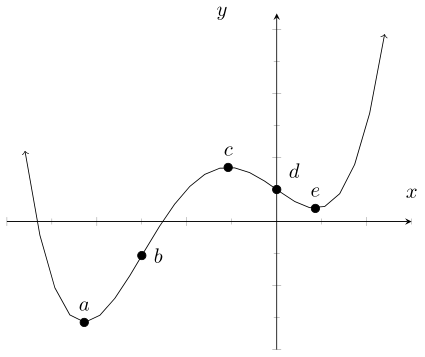
\includegraphics{ExamTwo-Picture0.png}
    \end{center}

    Based on the number of extrema, what is the smallest degree possible for the leading term of $f$?
    \begin{choices}
        \choiceShuffle[correct]{4}
        \choiceShuffle{3}
        \choiceShuffle{5}
        \choiceShuffle{6}
    \end{choices}
    }

\question{
    Consider the following graph:
    \begin{center}
        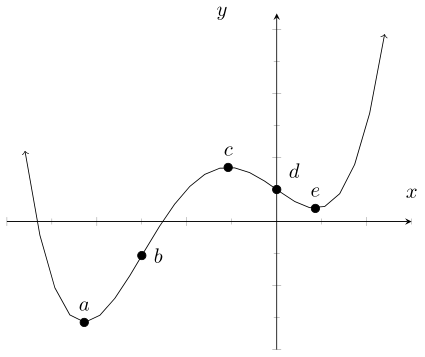
\includegraphics{ExamTwo-Picture1.png}
    \end{center}
    
    Within which of the following segments is the function \textbf{increasing} and concave \textbf{down}?
    \begin{choices}
    
        \choiceShuffle[correct]{Between b and c}
        \choiceShuffle{Between a and b}
        \choiceShuffle{Between c and d}
        \choiceShuffle{Between d and e}
        \choiceShuffle{To the right of e}
    \end{choices}
    }


\question{
    What is the leading coefficient of $(\sage{p1idFTAEf1}) + (\sage{p1idFTAEf2}) + (\sage{p1idFTAEf3}) + (\sage{p1idFTAEf4}) + (\sage{p1idFTAEf5})$?
    \begin{choices}
        \choiceShuffle[correct]{$\sage{p1idFTAEc1t}$}
        \choiceShuffle{$\sage{p1idFTAEc2t}$}
        \choiceShuffle{$\sage{p1idFTAEc3t}$}
        \choiceShuffle{$\sage{p1idFTAEc4t}$}
        \choiceShuffle{$\sage{p1idFTAEc5t}$}
    \end{choices}
    }

\question{
    Which of the following equations are polynomials?
    \begin{enumerate}\renewcommand{\labelenumii}{\Roman{enumii}:}
        \item $f(x) = x^2 + 1$
        \item $g(x) = \frac{1}{3}x^3 + 7$
        \item $h(x) = 7$
        \item $k(x) =x^3 + 3x^{\frac{1}{3}} + 1$
    \end{enumerate}
    \begin{choices}
        \choiceShuffle[correct]{I, II, and III Only.}
        \choiceShuffle{All of them are Polynomials.}
        \choiceShuffle{I and II Only.}
        \choiceShuffle{I Only.}
        \choiceShuffle{IV Only. }
    \end{choices}
    }% End question.



\question{
    Which of the following is the graph of $f(x) = (-x+2)^3 - 1$?
    \begin{choices}
        \choiceShuffle[correct]{
        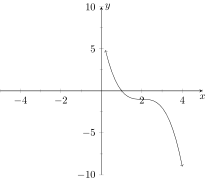
\includegraphics{ExamTwo-Picture2.png}
        }
        \choiceShuffle{
        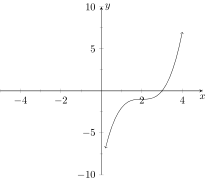
\includegraphics{ExamTwo-Picture3.png}
        }
        \choiceShuffle{
        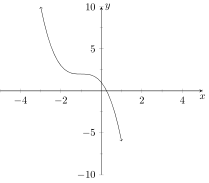
\includegraphics{ExamTwo-Picture4.png}
        }
        \choiceShuffle{
        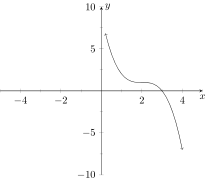
\includegraphics{ExamTwo-Picture5.png}
        }
        \choiceShuffle{
        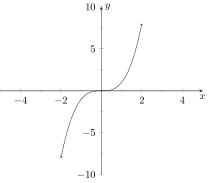
\includegraphics{ExamTwo-Picture6.png}
        }
    \end{choices}
    }



\question{
    Consider the polynomial $p(x) = \sage{p1idFTAMf4}$. How many zeros does this polynomial have counting multiplicity?
    \begin{choices}
        \choiceShuffle[correct]{$\sage{p1idFTAMans1}$}
        \choiceShuffle{$\sage{p1idFTAMans2}$}
        \choiceShuffle{$\sage{p1idFTAMans3}$}
        \choiceShuffle{$\sage{p1idFTAMans4}$}
        \choiceShuffle{$\sage{p1idFTAMans5}$}
    \end{choices}
    }

\question{
    How many zeros (and what type) does the polynomial $\sage{p2idFTAMf1}$ have?
    \begin{choices}
        \choiceShuffle[correct]{It has no real zeros, but according to FTA is has 2 complex zeros.}
        \choiceShuffle{It has no real zeros, so it must have complex zeros; but we cannot determine how many.}
        \choiceShuffle{According to FTA it has two real zeros and two complex zeros.}
        \choiceShuffle{According to FTA it has two real zeros and no complex zeros.}
        \choiceShuffle{Since it is degree two it has two zeros, one of which is complex, the other one is real.}
    \end{choices}
    }




\end{MCQuestions}
\end{document}